
%\newtheorem{definition}[subsection]{Definition}
%\newtheorem{example}[subsection]{Example}
\newtheorem{cor}[subsection]{Corollary}
\newtheorem{pro}[subsection]{Proposition}
\newtheorem{theo}[subsection]{Theorem}
\newtheorem{lem}[subsection]{Lemma}
%\newtheorem{rem}[subsection]{Remark}

\definecolor{main}{HTML}{5989cf}    % setting main color to be used
\definecolor{sub}{HTML}{cde4ff}     % setting sub color to be used

\tcbset{
    sharp corners,
    colback = white,
    before skip = 0.2cm,    % add extra space before the box
    after skip = 0.5cm      % add extra space after the box
}                           % setting global options for tcolorbox

% You can copy any following box you like to your code.
\newtcolorbox{boxA}{
    fontupper = \bf,
    boxrule = 1.5pt,
    colframe = black % frame color
}

\newtcolorbox{boxB}{
    fontupper = \bf\color{main}, % font color
    boxrule = 1.5pt,
    colframe = main,
    rounded corners,
    arc = 5pt   % corners roundness
}
\newtcolorbox{boxC}{
    colback = sub, % background color
    boxrule = 0pt  % no borders
}

\newtcolorbox{boxD}{
    colback = sub, 
    colframe = main, 
    boxrule = 0pt, 
    toprule = 3pt, % top rule weight
    bottomrule = 3pt % bottom rule weight
}

\hypersetup{
    colorlinks=true,
    linkcolor=blue,
    filecolor=magenta,      
    urlcolor=cyan,
    pdftitle={Overleaf Example},
    pdfpagemode=FullScreen,
    }

\urlstyle{same}


\coursetitle{\mtthreeiii}{MT303}
\developers{Wyclife Rao}
\reviewers{Dr Irene Sitawa}
\modulenumber{6}
\modulename{Numerical Integration and IVP for ODEs}

% courses
\thispagestyle{empty}
\begin{tikzpicture}[overlay,remember picture,font=\sffamily\bfseries]
 \draw[ultra thick,c4,name path=big arc] ([xshift=-2mm]current page.north) arc(150:285:11) coordinate[pos=0.225] (x0);
 \begin{scope}
  \clip ([xshift=-2mm]current page.north) arc(150:285:11) --(current page.north east);
  \fill[c4!50,opacity=0.25] ([xshift=4.55cm]x0) circle (4.55);
  \fill[c4!50,opacity=0.25] ([xshift=3.4cm]x0) circle (3.4);
  \fill[c4!50,opacity=0.25] ([xshift=2.25cm]x0) circle (2.25);
  \draw[ultra thick,c4!50] (x0) arc(-90:30:6.5);
  \draw[ultra thick,c4] (x0) arc(90:-30:8.75);
  \draw[ultra thick,c4!50,name path=arc1] (x0) arc(90:-90:4.675);
  \draw[ultra thick,c4!50] (x0) arc(90:-90:2.875);
  \path[name intersections={of=big arc and arc1,by=x1}];
  \draw[ultra thick,c4,name path=arc2] (x1) arc(135:-20:4.75);
  \draw[ultra thick,c4!50] (x1) arc(135:-20:8.75);
  \path[name intersections={of=big arc and arc2,by={aux,x2}}];
  \draw[ultra thick,c4!50] (x2) arc(180:50:2.25);
 \end{scope} 
 \path[decoration={text along path,text color=c4,
                 raise = -2.8ex,
                 text  along path,
                 text = {},%|\sffamily\bfseries|02/18/2019
                 text align = center,
             },
             decorate
         ] ([xshift=-2mm]current page.north) arc(150:245:11);
 %
 \newcommand\add{4cm}
 \begin{scope}%[shift={(5,0)}]
  \path[clip,postaction={fill=c3}]
  ([xshift=2cm+\add,yshift=-8cm]current page.center) rectangle ++ (4.6,7.7);
  \draw[c5,ultra thick,fill=c2] ([xshift=0.5cm+\add,yshift=-8cm]current page.center)
   ([xshift=0.5cm+\add,yshift=-8cm]current page.center)  arc(180:60:2)
    |- ++ (-3,6) --cycle;
  \draw[ultra thick,c5] ([xshift=-1.5cm+\add,yshift=-8cm]current page.center) 
  arc(180:0:2);
  \draw[ultra thick,c5] ([xshift=0.5cm+\add,yshift=-8cm]current page.center) 
  arc(180:0:2);
  \draw[ultra thick,c5] ([xshift=2.5cm+\add,yshift=-8cm]current page.center) 
  arc(180:0:2);
  \draw[ultra thick,c5] ([xshift=4.5cm+\add,yshift=-8cm]current page.center) 
  arc(180:0:2);
  \fill[white] ([xshift=2.5cm+\add,yshift=-8cm]current page.center) +(60:2) circle(1.5mm)
  node[above
  right=0mm,text=c5!80!black]{$\rho:=\dfrac{1+\sqrt{-3}}{2}$};
 \end{scope}
 %
 \fill[c1] ([xshift=2cm+\add,yshift=-8cm]current page.center) rectangle ++ (-30.7,7.7);
 \node[text=white,anchor=west,scale=2.3,inner sep=0pt] at
 ([xshift=-10cm,yshift=-1.8cm]current page.center) {\color{ulabgold} LEARNING};
 \node[text=white,anchor=west,scale=5,inner sep=0pt] at
 ([xshift=-10cm,yshift=-3.25cm]current page.center) {MODULE \dpmdnumber};
 \node[text=white,anchor=west,scale=2.5,inner sep=0pt,text width=.4\textwidth] at
 ([xshift=-10cm,yshift=-6cm]current page.center) {\dpmdname};
 \node[text=white,anchor=east,scale=2,inner sep=0pt] at
 ([xshift=5.7cm,yshift=-7.5cm]current page.center) {\color{ulabgold}The Open University of Kenya};
 %
% \draw[gray,line width=5mm] 
% ([xshift=2mm,yshift=-1mm]current page.south west) rectangle ([xshift=-2mm,yshift=1mm]current
% page.north east);
\end{tikzpicture}

%\newpage
\pagenumbering{roman}
\thispagestyle{empty}%firstpage


\begin{center}
\vspace*{2cm}
{\Huge\bf BACHELOR OF TECHNOLOGY EDUCATION}\\[3cm]  


%{\fontsize{80}{40}\selectfont \dpcoursecode}\\[2cm]
%
%{\fontsize{30}{40} \selectfont \dpcoursename}\\[2cm]

%\rule{\textwidth}{1pt}
%\vspace{2cm}

%{\fontsize{40}{40}\selectfont \bf Module~\dpmdnumber}\\[2cm]
%
%{\fontsize{30}{40}\selectfont \bf \dpmdname}\\

\vfill
\begin{flushright}
\begin{minipage}{.6\textwidth}
\begin{tcolorbox}%[text ]
\begin{tabular}{ll}%\hline
\subtitle{Developed by:}&\displaydevelopers\\
&\\
\subtitle{Reviewed by:}&\makecell[l]{\displayreviewers}\\
\end{tabular}
\end{tcolorbox}
\end{minipage}\hspace*{-3.5cm}
\end{flushright}
\vspace*{-2.5cm}
\end{center}

\newpage
\thispagestyle{empty}
\null
\vfill
{\renewcommand\arraystretch{1.5}
\begin{tabular}{|l|l|}\hline
\subtitle{Programme Title} & Bachelor of Technology Education \\\hline
\subtitle{Course Title} & \fullcoursename\\\hline
\subtitle{Learning Module number} & Module \dpmdnumber\\\hline
\subtitle{Learning module title} & \dpmdname \\\hline
\subtitle{Module Developer} & \displaydevelopers\\\hline
\subtitle{Reviewed by} & \displayreviewers\\\hline
%\subtitle{Vision} & \vision\\\hline
%\subtitle{Audience description} & \\\hline
\end{tabular}}
\clearpage

%\section{COURSE LEARNING GUIDE}


\subsection*{Preparing for Online and Distance Learning}

This course offers you the opportunity to enter an online space where you can engage with fellow students at the university. The online forums, exercises, tasks and materials have been designed by the course facilitators in such a way that you can draw directly from their knowledge and share in their scholarly interest in online learning and assessment

We hope you will use your access to this virtual classroom to raise all your questions on the course module, to build a network great learners and to share your own thoughts and experiences to the benefit of your fellow students.

   
There are a number of steps you can take to ensure you are well prepared to make the most of this learning opportunity. This resource should prompt you to consider the following:


 \begin{enumerate}[label=\cb$\square$]
   \item How can you best prepare the space where you expect you will spend most of your time engaging in online learning (i.e. in your home or office, or even during your commute to work or whilst traveling)?
  \item   What can you do to ensure you keep working through the course material, even when you do not have Internet access?
    \item How can you familiarise yourself with the course layout, in order to be able to navigate through the steps with ease?
    \item What are the communication strategies and best practices you could consider to best engage with your fellow students and the course facilitators?
    \item What do you do when you need academic or technical support?

 \end{enumerate} 

\subsection*{General Module Guide}

The authors of this module believe that imparting knowledge should always be a mutual relationship between the students and the teachers. Students can actively construct knowledge through experiences gained in reading and answering the learning modules.

You should take time to read everything written in the module, actively and religiously solve all the exercises included to finish this course and be able to gain all the competencies and skills expected to demonstrate the learning outcomes as stated in this course. If you finish with full confidence that you understand and can apply all the knowledge you gain in this course, then you are sure to succeed in tackling the next higher subjects in your chosen course.

In this course, you will be taught not only the knowledge you need to demonstrate your learning outcomes, but you will also gain discipline, perseverance, higher thinking skills, and resourcefulness that would help strengthen your foundation to succeed in life. To successfully finish the course, you must follow the guides set forth in using this module.


\begin{description}[{format=\textcolor{ulabblue}}]
\item[STUDY ENVIRONMENT.]\leavevmode\\
Before engaging into the module, make sure that you are comfortable enough and diminish distractions. Make sure that you develop a study routine to perform and accomplish all the activities set forth by the module.
%\newpage

\item[MODE OF DELIVERY.]\leavevmode\\
Students are required to get a access a digitised copy of the module from the Virtue Learning Environment. As an open and distance learner, you should be able to learn independently and optimise the learning modes and environment available to you as much of  the delivery of all the lessons will be done asynchronously. Your success will greatly depend on your self-motivation and discipline to get your work done without your instructor to remind you from time to time.

\item[STUDY SCHEDULE.] \leavevmode\\
Remember that you have other subjects to attend to, hence, you must manage your time so that you will not be left behind in any of them. Create your own learning plan for each course to make sure that you can perform all the activities. Do not procrastinate your work, remember that time wasted can never be retrieved back. Make sure that even if you are at home, you are a student enrolled in a program, where the learning of all its courses greatly depends on your will to learn as the materials you need are all in your hands. So always be aware of your daily tasks.

\item[PRACTICE EXERCISE.]\leavevmode\\
To measure your learning from your reading, you are given practice exercises which you are supposed to answer daily. This will prepare you in performing your main task.

\item[ONLINE GROUP CHAT.]\leavevmode\\
I am going to create an online Discussion Forum and QA Forum  on the VLE.  This will serve as a room for discussion on the topics and activities found in your module.

\item[RECOMMENDED REFERENCES FOR SUPPLEMENTARY READING.]\leavevmode\\
You are given links that you need to access online. These links are online references such as e-books, online activities, and tutorial videos of the topic. These are other references you can use to further understand the topic and gain additional knowledge and skills.

\item[MAIN TASK.]\leavevmode\\
You are given a task that will require you to apply the knowledge and skills you learned from the module. This can be a group or individual activity which will measure your higher order thinking skills you acquired throughout the topic.

\item[RUBRICS. ]\leavevmode\\
This is a tool to guide you in performing your main task. Through this, you will be able to know the specific indicators that should be found in your task. This is to assess your constructive behaviour towards your learning application. You will be rated according to a 4-point scale shown below.
\begin{center}
{\color{ulabgold} \bf 4 − Excellent\quad\quad   3 −Good\quad\quad    2 − Fair \quad\quad  1 −Poor}
\end{center}
\item[REFLECTIONS.]\leavevmode\\
Writing your reflection will be a passageway to express your experiential learning in using this module. In your honest recall, write everything that you think happened to you during your learning experience in this module. Use the guide questions below:
\begin{description}[{format=\textcolor{ulabblue}}]
\item[First paragraph. ]\leavevmode\\
How was your learning experience? Maybe you can consider describing the effect of the parts of the module (sequence, discussions, examples, practice exercises, online activities, and the main task) in your learning experience. You can point out the strength and weakness of each part so that we can consider it for future improvement of this instructional material.
\item[Second paragraph.  ]\leavevmode\\
What did you learn? Did you successfully acquire the learning outcomes?

\item[Third paragraph.]\leavevmode\\
How can you use what you learned in the future?
\end{description}
\end{description}

\section{ASSESSMENT  TASKS \& EXAMINATION   RULES AND GUIDELINES}

\begin{enumerate}[label=\cb\arabic*.]
\item {\cb SUBMISSION OF ASSESSMENT TASTS.}

Since mathematical skills are best acquired through constant practice, you are encouraged to answer at least two (2) exercises a day. These practice exercises will not be graded but it will help you develop your thinking skills which will prepare you in the performance of your main tasks. You are required to submit your practice exercises every week.
\begin{center} {\cg Usually submission deadlines are set on Saturday 11:59PM EAT} \end{center}

\item  {\cb GROUP CHAT.}

You can post questions, solutions, and comment to other's post. Please be reminded that our group chat is exclusive only for discussion on topics related to this course. Everyone is required to actively participate in the discussions. Also, trolling is highly discouraged. Always observe proper online etiquettes when participating in discussions.
\begin{center} {\cb RULE OF THUMB: ALWAYS THINK BEFORE YOU CLICK} \end{center}

\item  {\cb MAIN TASK. }

Complete documentation during the preparation of your task is required to ensure that every member of the group participated and contributed in the task. May it be photos or screenshots of your virtual meetings or group works. You are going to submit it as attachment of your main task the same way as the practice exercises.



\item {\cb RECOMMENDED REFERENCES FOR SUPPLEMENTARY READING.} 

You can explore online for other references that is related to the topic to gain additional information about the topic. Do not share or post inappropriate materials online or even privately.
\end{enumerate}

\subsection*{Requirements to pass the course}

Compiled Continuous  Assignment/Activities and Tasks  with Final Performance Examination.

\subtitle{Grading System}
\begin{center}
{\renewcommand\arraystretch{1.5}
\begin{tabular}{|l|c|}\hline
Continuous Activities and Tasks  &  50\%\\\hline
Final Performance Examination. &  50\%\\\hline
\end{tabular}
}
\end{center}
%\newpage










%\subsection{INTRODUCTORY MESSAGE}

%A warm welcome to \;  \fullcoursename, {\bf Module on \dpmdname}.



%By this module learning resource, we aim to enable you  achieve the relevant competencies, depict skill, action and purpose successfully. 
 

%It has been designed to provide you with fun and meaningful opportunities for guided and independent learning at your own pace and time. You will be enabled to process the contents of the learning material while being an active learner. Your academic success lies in your own hands.  This module has the following parts and corresponding icons:





{
\renewcommand\arraystretch{4}
\begin{longtblr}{
width=\linewidth,
 colspec={ Q[1,c,f] Q[1.5,r,m] Q[4,l,m] },
%row{1} = { font=\bfseries },
% rowhead = 1,
  caption={ }, 
  label={ },
  rowsep = 4pt,
  hlines = {ulabblue!20, 1pt},
  vlines = {ulabblue!20, 1pt},
}

\includegraphics[width=2cm]{img/audience} & {\bf AUDIENCE}  &  This is a description of a target audience.   \\
{\fontsize{40}{30}\selectfont\color{ulabblue}\faCogs}& {\bf MODULE DESCRIPTION} & 
This part explains the importance of the topics discussed in the module. It will also give you a sneak peek of what you will learn and what is expected from you at the end of the module.\\

\includegraphics[width=2cm]{img/target.png} &  {\bf  EXPECTATION} & These are what you will be able to know after completing the lessons in the module\\

\includegraphics[width=2cm]{img/preactivities} & {\bf PRE-ACTIVITY} &
This activity is to get you set, activate and engage schema to learn the module. Through this activity, you will know the relevance of this activity to the topic that will be discussed in the module.\\

\includegraphics[width=2cm]{img/pretest} &  {\bf PRE - ASSESSMENT} & This will measure your prior knowledge and the concepts to be mastered throughout the lesson. \\

\includegraphics[width=1.7cm]{img/rewind} &  {\bf  RECAP} & This section will measure what learnings and skills that you understand from the previous lesson.\\

\includegraphics[width=1.5cm]{img/lesson} &  {\bf  LESSON} & This section will discuss the topic for this module.\\

\includegraphics[width=2cm]{img/activities} &  {\bf  ACTIVITIES} & This is a set of activities you will perform.\\

\includegraphics[width=2cm]{img/summary} &  {\bf  WRAP UP} & This section summarizes the concepts and applications of the lessons.\\

\includegraphics[width=2cm]{img/discussion}& {\bf DISCUSSIONS} &
This is the meat of the module. The discussion is aligned to the topic learning outcomes that is expected of you to acquire at the end of the module.\\

\includegraphics[width=1.8cm]{img/value} &  {\bf  VALUING} & This part will check the integration of values in the learning competency you will take home.\\

\includegraphics[width=1.8cm]{img/posttest} &  {\bf  POST - ASSESSMENT} & This will measure how much you have learned from the entire module.\\

\includegraphics[width=1.8cm]{img/selfreflect} & {\bf REFLECTION }
&
This part is for you to share your thoughts by writing your reflection, make sure to check your grammar and spelling to ensure the readability and so that it will not alter the thought being delivered. 
\end{longtblr}
}









%\vfill

\audience
\begin{oldactivity}{Audience Description}{
\includegraphics[width=22mm]{img/audience}}{}
This module is offered to all students taking the Bachelor of Technology Education. As an open and distance learner, you should be able to learn independently and optimise the learning modes and environment available to you. Before you begin this course, please confirm the course material, the course requirements and how the course is conducted.
\end{oldactivity}
%\newpage
\pagenumbering{arabic}



\mddescription
This module guides you into a detailed discussion of the concepts of numerical integration. Specifically you will learn about
\begin{itemize}
\item multiple integrals
\item improper integrals
\item the elementary theory of initial-value problems
\item Euler's method 
\end{itemize}
%\expectations
%\begin{objenumerate}
%
%\end{objenumerate}

\begin{mlos}
\item Identify the characteristics of multiple and improper integrals.
\item Describe numerical methods for solving multiple and improper integrals.
\item Solve first-order ODEs using Euler’s numerical method.
\item Construct numerical solutions of initial value problems.
\end{mlos}

\section{Multiple Integrals}
\videolesson
\begin{selfvideo}[1]
%LESSON 3: 
This video presents a discussion on multiple integrals. Follow the discussion and then solve the problems in the subsequent quiz.
\end{selfvideo}

The techniques discussed in the previous sections can be modified for use in the approximation of multiple integrals. Consider the double integral

$$
\iint_{R} f(x, y) d A,
$$

where $R=\{(x, y) \mid a \leq x \leq b, c \leq y \leq d\}$, for some constants $a, b, c$, and $d$, is a rectangular region in the plane. (See Figure \ref{fig:multipleintegral1}.)

%Figure 4.18\\
\begin{figure}
\centering
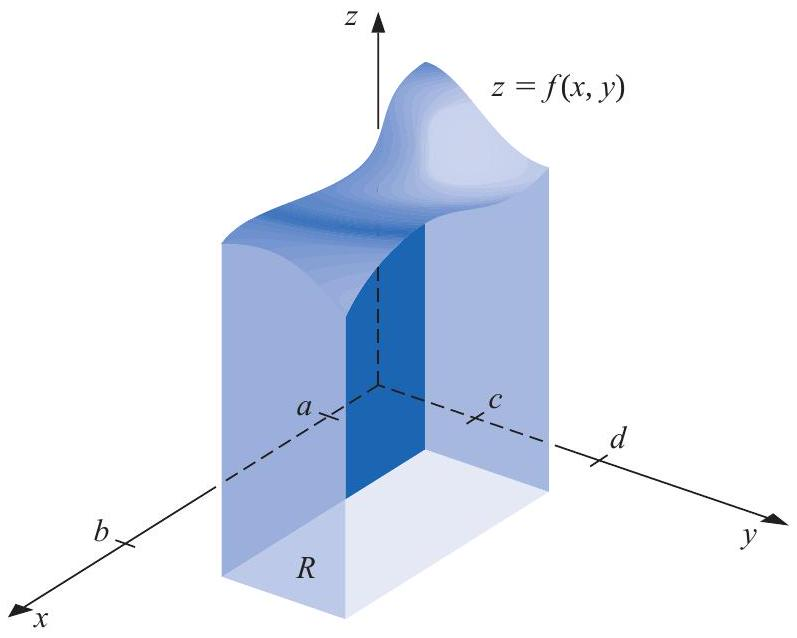
\includegraphics[width=10cm]{2025_05_15_85b7f7df47271a498e1dg-63}
\caption{\scriptsize Figure $1$}
\label{fig:multipleintegral1}
\end{figure}

The following illustration shows how the Composite Trapezoidal rule using two subintervals in each coordinate direction would be applied to this integral.

Illustration Writing the double integral as an iterated integral gives

$$
\iint_{R} f(x, y) d A=\int_{a}^{b}\left(\int_{c}^{d} f(x, y) d y\right) d x .
$$

To simplify notation, let $k=(d-c) / 2$ and $h=(b-a) / 2$. Apply the Composite Trapezoidal rule to the interior integral to obtain

$$
\int_{c}^{d} f(x, y) d y \approx \frac{k}{2}\left[f(x, c)+f(x, d)+2 f\left(x, \frac{c+d}{2}\right)\right]
$$

This approximation is of order $O\left((d-c)^{3}\right)$. Then apply the Composite Trapezoidal rule again to approximate the integral of this function of $x$ :

$$
\begin{aligned}
\int_{a}^{b}\left(\int_{c}^{d} f(x, y) d y\right) d x \approx & \int_{a}^{b}\left(\frac{d-c}{4}\right)\left[f(x, c)+2 f\left(x, \frac{c+d}{2}\right)+f(d)\right] d x \\
= & \frac{b-a}{4}\left(\frac{d-c}{4}\right)\left[f(a, c)+2 f\left(a, \frac{c+d}{2}\right)+f(a, d)\right] \\
& +\frac{b-a}{4}\left(2 ( \frac { d - c } { 4 } ) \left[f\left(\frac{a+b}{2}, c\right)\right.\right. \\
& \left.\left.+2 f\left(\frac{a+b}{2}, \frac{c+d}{2}\right)+\left(\frac{a+b}{2}, d\right)\right]\right) \\
& +\frac{b-a}{4}\left(\frac{d-c}{4}\right)\left[f(b, c)+2 f\left(b, \frac{c+d}{2}\right)+f(b, d)\right] \\
%= & \frac{(b-a)(d-c)}{16}[f(a, c)+f(a, d)+f(b, c)+f(b, d) \\
%& +2\left(f\left(\frac{a+b}{2}, c\right)+f\left(\frac{a+b}{2}, d\right)+f\left(a, \frac{c+d}{2}\right)\right. \\
%& \left.\left.+f\left(b, \frac{c+d}{2}\right)\right)+4 f\left(\frac{a+b}{2}, \frac{c+d}{2}\right)\right]
\end{aligned}
$$

Therefore
$$
\begin{aligned}
\int_{a}^{b}\left(\int_{c}^{d} f(x, y) d y\right) d x &\approx 
%\int_{a}^{b}\left(\frac{d-c}{4}\right)\left[f(x, c)+2 f\left(x, \frac{c+d}{2}\right)+f(d)\right] d x \\
%= & \frac{b-a}{4}\left(\frac{d-c}{4}\right)\left[f(a, c)+2 f\left(a, \frac{c+d}{2}\right)+f(a, d)\right] \\
%& +\frac{b-a}{4}\left(2 ( \frac { d - c } { 4 } ) \left[f\left(\frac{a+b}{2}, c\right)\right.\right. \\
%& \left.\left.+2 f\left(\frac{a+b}{2}, \frac{c+d}{2}\right)+\left(\frac{a+b}{2}, d\right)\right]\right) \\
%& +\frac{b-a}{4}\left(\frac{d-c}{4}\right)\left[f(b, c)+2 f\left(b, \frac{c+d}{2}\right)+f(b, d)\right] \\
\frac{(b-a)(d-c)}{16}[f(a, c)+f(a, d)+f(b, c)+f(b, d) \\
& +2\left(f\left(\frac{a+b}{2}, c\right)+f\left(\frac{a+b}{2}, d\right)+f\left(a, \frac{c+d}{2}\right)\right. \\
& \left.\left.+f\left(b, \frac{c+d}{2}\right)\right)+4 f\left(\frac{a+b}{2}, \frac{c+d}{2}\right)\right]
\end{aligned}
$$

This approximation is of order $O\left((b-a)(d-c)\left[(b-a)^{2}+(d-c)^{2}\right]\right)$. Figure \ref{fig:multipleintegral2} shows a grid with the number of functional evaluations at each of the nodes used in the approximation.

%Figure 4.19\\
\begin{figure}[h]
\centering
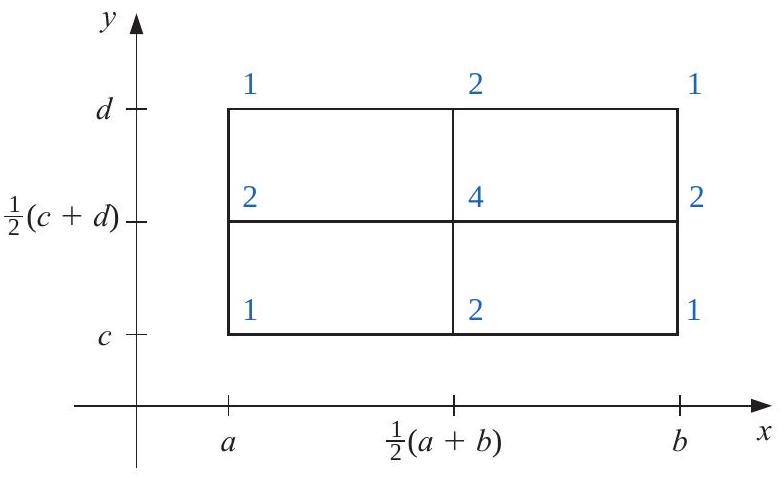
\includegraphics[width=10cm]{2025_05_15_85b7f7df47271a498e1dg-64}
\caption{\scriptsize Figure $2$}
\label{fig:multipleintegral2}
\end{figure}

As the illustration shows, the procedure is quite straightforward. But the number of function evaluations grows with the square of the number required for a single integral. In a practical situation we would not expect to use a method as elementary as the Composite Trapezoidal rule. Instead we will employ the Composite Simpson's rule to illustrate the general approximation technique, although any other composite formula could be used in its place.

To apply the Composite Simpson's rule, we divide the region $R$ by partitioning both $[a, b]$ and $[c, d]$ into an even number of subintervals. To simplify the notation, we choose even integers $n$ and $m$ and partition $[a, b]$ and $[c, d]$ with the evenly spaced mesh points $x_{0}, x_{1}, \ldots, x_{n}$ and $y_{0}, y_{1}, \ldots, y_{m}$, respectively. These subdivisions determine step sizes $h=$ $(b-a) / n$ and $k=(d-c) / m$. Writing the double integral as the iterated integral

$$
\iint_{R} f(x, y) d A=\int_{a}^{b}\left(\int_{c}^{d} f(x, y) d y\right) d x
$$

we first use the Composite Simpson's rule to approximate

$$
\int_{c}^{d} f(x, y) d y
$$

treating $x$ as a constant.

Let $y_{j}=c+j k$, for each $j=0,1, \ldots, m$. Then

$$
\begin{aligned}
\int_{c}^{d} f(x, y) d y= & \frac{k}{3}\left[f\left(x, y_{0}\right)+2 \sum_{j=1}^{(m / 2)-1} f\left(x, y_{2 j}\right)+4 \sum_{j=1}^{m / 2} f\left(x, y_{2 j-1}\right)+f\left(x, y_{m}\right)\right] \\
& -\frac{(d-c) k^{4}}{180} \frac{\partial^{4} f}{\partial y^{4}}(x, \mu)
\end{aligned}
$$

for some $\mu$ in ( $c, d$ ). Thus

$$
\begin{aligned}
\int_{a}^{b} \int_{c}^{d} f(x, y) d y d x= & \frac{k}{3}\left[\int_{a}^{b} f\left(x, y_{0}\right) d x+2 \sum_{j=1}^{(m / 2)-1} \int_{a}^{b} f\left(x, y_{2 j}\right) d x\right. \\
& \left.+4 \sum_{j=1}^{m / 2} \int_{a}^{b} f\left(x, y_{2 j-1}\right) d x+\int_{a}^{b} f\left(x, y_{m}\right) d x\right] \\
& -\frac{(d-c) k^{4}}{180} \int_{a}^{b} \frac{\partial^{4} f}{\partial y^{4}}(x, \mu) d x
\end{aligned}
$$

Composite Simpson's rule is now employed on the integrals in this equation. Let $x_{i}=a+i h$, for each $i=0,1, \ldots, n$. Then for each $j=0,1, \ldots, m$, we have

$$
\begin{aligned}
\int_{a}^{b} f\left(x, y_{j}\right) d x= & \frac{h}{3}\left[f\left(x_{0}, y_{j}\right)+2 \sum_{i=1}^{(n / 2)-1} f\left(x_{2 i}, y_{j}\right)+4 \sum_{i=1}^{n / 2} f\left(x_{2 i-1}, y_{j}\right)+f\left(x_{n}, y_{j}\right)\right] \\
& -\frac{(b-a) h^{4}}{180} \frac{\partial^{4} f}{\partial x^{4}}\left(\xi_{j}, y_{j}\right)
\end{aligned}
$$

for some $\xi_{j}$ in ( $a, b$ ). The resulting approximation has the form

$$
\begin{aligned}
\int_{a}^{b} \int_{c}^{d} f(x, y) d y d x \approx & \frac{h k}{9}\left\{\left[f\left(x_{0}, y_{0}\right)+2 \sum_{i=1}^{(n / 2)-1} f\left(x_{2 i}, y_{0}\right)+4 \sum_{i=1}^{n / 2} f\left(x_{2 i-1}, y_{0}\right)+f\left(x_{n}, y_{0}\right)\right]\right. \\
& +2\left[\sum_{j=1}^{(m / 2)-1} f\left(x_{0}, y_{2 j}\right)+2 \sum_{j=1}^{(m / 2)-1} \sum_{i=1}^{(n / 2)-1} f\left(x_{2 i}, y_{2 j}\right)\right. \\
& \left.+4 \sum_{j=1}^{(m / 2)-1} \sum_{i=1}^{n / 2} f\left(x_{2 i-1}, y_{2 j}\right)+\sum_{j=1}^{(m / 2)-1} f\left(x_{n}, y_{2 j}\right)\right] \\
& +4\left[\sum_{j=1}^{m / 2} f\left(x_{0}, y_{2 j-1}\right)+2 \sum_{j=1}^{m / 2} \sum_{i=1}^{(n / 2)-1} f\left(x_{2 i}, y_{2 j-1}\right)\right. \\
& \left.+4 \sum_{j=1}^{m / 2} \sum_{i=1}^{n / 2} f\left(x_{2 i-1}, y_{2 j-1}\right)+\sum_{j=1}^{m / 2} f\left(x_{n}, y_{2 j-1}\right)\right] \\
& \left.+\left[f\left(x_{0}, y_{m}\right)+2 \sum_{i=1}^{(n / 2)-1} f\left(x_{2 i}, y_{m}\right)+4 \sum_{i=1}^{n / 2} f\left(x_{2 i-1}, y_{m}\right)+f\left(x_{n}, y_{m}\right)\right]\right\}
\end{aligned}
$$

The error term $E$ is given by

$$
\begin{aligned}
E= & \frac{-k(b-a) h^{4}}{540}\left[\frac{\partial^{4} f}{\partial x^{4}}\left(\xi_{0}, y_{0}\right)+2 \sum_{j=1}^{(m / 2)-1} \frac{\partial^{4} f}{\partial x^{4}}\left(\xi_{2 j}, y_{2 j}\right)+4 \sum_{j=1}^{m / 2} \frac{\partial^{4} f}{\partial x^{4}}\left(\xi_{2 j-1}, y_{2 j-1}\right)\right. \\
& \left.+\frac{\partial^{4} f}{\partial x^{4}}\left(\xi_{m}, y_{m}\right)\right]-\frac{(d-c) k^{4}}{180} \int_{a}^{b} \frac{\partial^{4} f}{\partial y^{4}}(x, \mu) d x
\end{aligned}
$$

If $\partial^{4} f / \partial x^{4}$ is continuous, the Intermediate Value Theorem can be repeatedly applied to show that the evaluation of the partial derivatives with respect to $x$ can be replaced by a common value and that

$$
E=\frac{-k(b-a) h^{4}}{540}\left[3 m \frac{\partial^{4} f}{\partial x^{4}}(\bar{\eta}, \bar{\mu})\right]-\frac{(d-c) k^{4}}{180} \int_{a}^{b} \frac{\partial^{4} f}{\partial y^{4}}(x, \mu) d x
$$

for some $(\bar{\eta}, \bar{\mu})$ in $R$. If $\partial^{4} f / \partial y^{4}$ is also continuous, the Weighted Mean Value Theorem for Integrals implies that

$$
\int_{a}^{b} \frac{\partial^{4} f}{\partial y^{4}}(x, \mu) d x=(b-a) \frac{\partial^{4} f}{\partial y^{4}}(\hat{\eta}, \hat{\mu})
$$

for some ( $\hat{\eta}, \hat{\mu}$ ) in $R$. Because $m=(d-c) / k$, the error term has the form

$$
E=\frac{-k(b-a) h^{4}}{540}\left[3 m \frac{\partial^{4} f}{\partial x^{4}}(\bar{\eta}, \bar{\mu})\right]-\frac{(d-c)(b-a)}{180} k^{4} \frac{\partial^{4} f}{\partial y^{4}}(\hat{\eta}, \hat{\mu})
$$

which simplifies to

$$
E=-\frac{(d-c)(b-a)}{180}\left[h^{4} \frac{\partial^{4} f}{\partial x^{4}}(\bar{\eta}, \bar{\mu})+k^{4} \frac{\partial^{4} f}{\partial y^{4}}(\hat{\eta}, \hat{\mu})\right]
$$

for some $(\bar{\eta}, \bar{\mu})$ and $(\hat{\eta}, \hat{\mu})$ in $R$.

\begin{example}\label{examp:multipleintegral1}
Use Composite Simpson's rule with $n=4$ and $m=2$ to approximate

$$
\int_{1.4}^{2.0} \int_{1.0}^{1.5} \ln (x+2 y) d y d x
$$
\end{example}

\begin{mysolution}
The step sizes for this application are $h=(2.0-1.4) / 4=0.15$ and $k=$ $(1.5-1.0) / 2=0.25$. The region of integration $R$ is shown in Figure 4.20, together with the nodes $\left(x_{i}, y_{j}\right)$, where $i=0,1,2,3,4$ and $j=0,1,2$. It also shows the coefficients $w_{i, j}$ of $f\left(x_{i}, y_{i}\right)=\ln \left(x_{i}+2 y_{i}\right)$ in the sum that gives the Composite Simpson's rule approximation to the integral.

\begin{center}
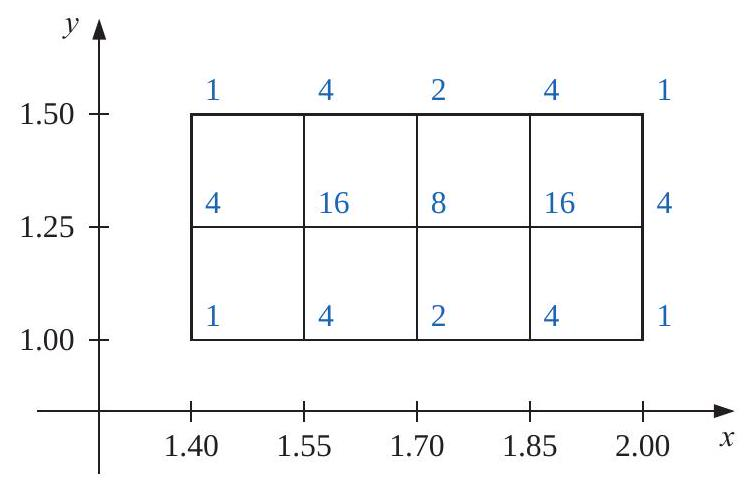
\includegraphics[width=10cm]{2025_05_15_85b7f7df47271a498e1dg-67}
\end{center}

The approximation is

$$
\begin{aligned}
\int_{1.4}^{2.0} \int_{1.0}^{1.5} \ln (x+2 y) d y d x & \approx \frac{(0.15)(0.25)}{9} \sum_{i=0}^{4} \sum_{j=0}^{2} w_{i, j} \ln \left(x_{i}+2 y_{j}\right) \\
& =0.4295524387
\end{aligned}
$$

We have

$$
\frac{\partial^{4} f}{\partial x^{4}}(x, y)=\frac{-6}{(x+2 y)^{4}} \quad \text { and } \quad \frac{\partial^{4} f}{\partial y^{4}}(x, y)=\frac{-96}{(x+2 y)^{4}}
$$

and the maximum values of the absolute values of these partial derivatives occur on $R$ when $x=1.4$ and $y=1.0$. So the error is bounded by

$$
|E| \leq \frac{(0.5)(0.6)}{180}\left[(0.15)^{4} \max _{(x, y) \operatorname{in} R} \frac{6}{(x+2 y)^{4}}+(0.25)^{4} \max _{(x, y) \operatorname{in} R} \frac{96}{(x+2 y)^{4}}\right] \leq 4.72 \times 10^{-6}
$$

The actual value of the integral to ten decimal places is

$$
\int_{1.4}^{2.0} \int_{1.0}^{1.5} \ln (x+2 y) d y d x=0.4295545265
$$

so the approximation is accurate to within $2.1 \times 10^{-6}$\qed
\end{mysolution}

The same techniques can be applied for the approximation of triple integrals as well as higher integrals for functions of more than three variables. The number of functional evaluations required for the approximation is the product of the number of functional evaluations required when the method is applied to each variable.

\subsection*{Gaussian Quadrature for Double Integral Approximation}
To reduce the number of functional evaluations, more efficient methods such as Gaussian quadrature, Romberg integration, or Adaptive quadrature can be incorporated in place of the Newton-Cotes formulas. The following example illustrates the use of Gaussian quadrature for the integral considered in Example 1.

\begin{example}
Use Gaussian quadrature with $n=3$ in both dimensions to approximate the integral

$$
\int_{1.4}^{2.0} \int_{1.0}^{1.5} \ln (x+2 y) d y d x
$$
\end{example}

\begin{mysolution}
Before employing Gaussian quadrature to approximate this integral, we need to transform the region of integration

$$
R=\{(x, y) \mid 1.4 \leq x \leq 2.0,1.0 \leq y \leq 1.5\}
$$

into

$$
\hat{R}=\{(u, v) \mid-1 \leq u \leq 1,-1 \leq v \leq 1\} .
$$

The linear transformations that accomplish this are

$$
u=\frac{1}{2.0-1.4}(2 x-1.4-2.0) \quad \text { and } \quad v=\frac{1}{1.5-1.0}(2 y-1.0-1.5),
$$

or, equivalently, $x=0.3 u+1.7$ and $y=0.25 v+1.25$. Employing this change of variables gives an integral on which Gaussian quadrature can be applied:

$$
\int_{1.4}^{2.0} \int_{1.0}^{1.5} \ln (x+2 y) d y d x=0.075 \int_{-1}^{1} \int_{-1}^{1} \ln (0.3 u+0.5 v+4.2) d v d u
$$

The Gaussian quadrature formula for $n=3$ in both $u$ and $v$ requires that we use the nodes

$$
u_{1}=v_{1}=r_{3,2}=0, \quad u_{0}=v_{0}=r_{3,1}=-0.7745966692,
$$

and

$$
u_{2}=v_{2}=r_{3,3}=0.7745966692
$$

The associated weights are $c_{3,2}=0 . \overline{8}$ and $c_{3,1}=c_{3,3}=0 . \overline{5}$. (These are given in Table 4.12 on page 232.) The resulting approximation is

$$
\begin{aligned}
\int_{1.4}^{2.0} \int_{1.0}^{1.5} \ln (x+2 y) d y d x & \approx 0.075 \sum_{i=1}^{3} \sum_{j=1}^{3} c_{3, i} c_{3, j} \ln \left(0.3 r_{3, i}+0.5 r_{3, j}+4.2\right) \\
& =0.4295545313
\end{aligned}
$$

Although this result requires only $9$ functional evaluations compared to $15$ for the Composite Simpson's rule considered in Example \ref{examp:multipleintegral1}, it is accurate to within $4.8 \times 10^{-9}$, compared to $2.1 \times 10^{-6}$ accuracy in Example \ref{examp:multipleintegral1}.\qed
\end{mysolution}

\subsection*{Non-Rectangular Regions}
The use of approximation methods for double integrals is not limited to integrals with rectangular regions of integration. The techniques previously discussed can be modified to approximate double integrals of the form


\begin{equation}\label{eqn:nonrectangle1}
\int_{a}^{b} \int_{c(x)}^{d(x)} f(x, y) d y d x \tag{4.42}
\end{equation}


or


\begin{equation}\label{eqn:nonrectangle2}
\int_{c}^{d} \int_{a(y)}^{b(y)} f(x, y) d x d y . \tag{4.43}
\end{equation}


In fact, integrals on regions not of this type can also be approximated by performing appropriate partitions of the region. (See Exercise 10.)

To describe the technique involved with approximating an integral in the form

$$
\int_{a}^{b} \int_{c(x)}^{d(x)} f(x, y) d y d x
$$

we will use the basic Simpson's rule to integrate with respect to both variables. The step size for the variable $x$ is $h=(b-a) / 2$, but the step size for $y$ varies with $x$ (see Figure 4.21) and is written

$$
k(x)=\frac{d(x)-c(x)}{2} .
$$

%Figure 4.21\\
\begin{figure}[h]
\centering
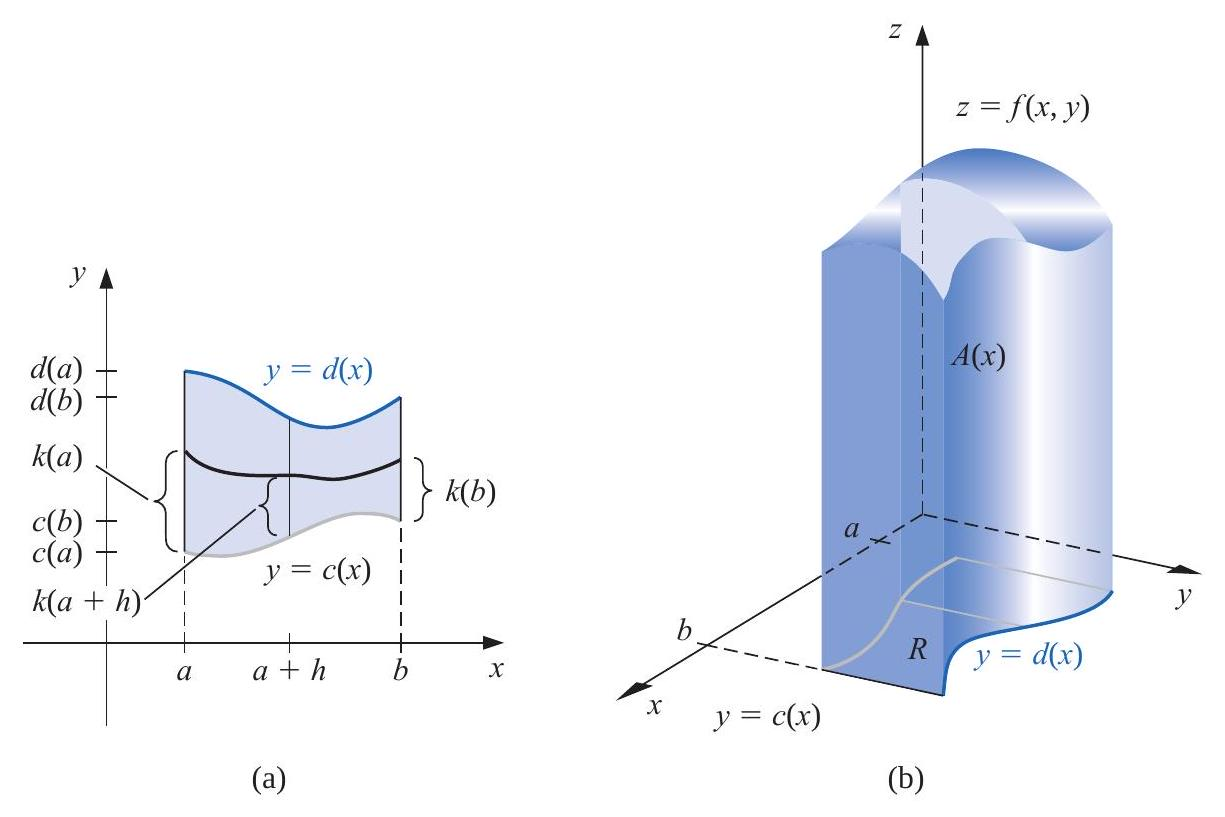
\includegraphics[width=13cm]{2025_05_15_85b7f7df47271a498e1dg-69}
\caption{\scriptsize Figure $3$: Non-rectangular region}
\label{fig:nonrectangle1}
\end{figure}

This gives

$$
\begin{aligned}
\int_{a}^{b} \int_{c(x)}^{d(x)} f(x, y) d y d x \approx & \int_{a}^{b} \frac{k(x)}{3}[f(x, c(x))+4 f(x, c(x)+k(x))+f(x, d(x))] d x \\
\approx & \frac{h}{3}\left\{\frac{k(a)}{3}[f(a, c(a))+4 f(a, c(a)+k(a))+f(a, d(a))]\right. \\
& +\frac{4 k(a+h)}{3}[f(a+h, c(a+h))+4 f(a+h, c(a+h) \\
& +k(a+h))+f(a+h, d(a+h))] \\
& \left.+\frac{k(b)}{3}[f(b, c(b))+4 f(b, c(b)+k(b))+f(b, d(b))]\right\}
\end{aligned}
$$

%Algorithm 4.4 applies the Composite Simpson's rule to an integral in the form (4.42). Integrals in the form (4.43) can, of course, be handled similarly.
%
%\section*{Simpson's Double Integral}
%To approximate the integral
%
%$$
%I=\int_{a}^{b} \int_{c(x)}^{d(x)} f(x, y) d y d x
%$$
%
%INPUT endpoints $a, b$ : even positive integers $m, n$.\\
%OUTPUT approximation $J$ to $I$.\\
%Step 1 Set $h=(b-a) / n$;\\
%$J_{1}=0 ; \quad($ End terms.$)$\\
%$J_{2}=0 ; \quad$ (Even terms.)\\
%$J_{3}=0 . \quad$ (Odd terms.)\\
%Step 2 For $i=0,1, \ldots, n$ do Steps 3-8.\\
%Step 3 Set $x=a+i h$; (Composite Simpson's method for $x$.)
%
%$$
%\begin{aligned}
%& H X=(d(x)-c(x)) / m ; \\
%& K_{1}=f(x, c(x))+f(x, d(x)) ; \quad(\text { End terms } .) \\
%& K_{2}=0 ; \quad(\text { Even terms } .) \\
%& K_{3}=0 . \quad(\text { Odd terms } .)
%\end{aligned}
%$$
%
%Step 4 For $j=1,2, \ldots, m-1$ do Step 5 and 6.\\
%Step 5 Set $y=c(x)+j H X$;
%
%$$
%Q=f(x, y)
%$$
%
%Step 6 If $j$ is even then set $K_{2}=K_{2}+Q$ else set $K_{3}=K_{3}+Q$.
%
%Step 7 Set $L=\left(K_{1}+2 K_{2}+4 K_{3}\right) H X / 3$.\\
%$\left(L \approx \int_{c\left(x_{i}\right)}^{d\left(x_{i}\right)} f\left(x_{i}, y\right) d y\right.$ by the Composite Simpson's method.)\\
%Step 8 If $i=0$ or $i=n$ then set $J_{1}=J_{1}+L$ else if $i$ is even then set $J_{2}=J_{2}+L$ else set $J_{3}=J_{3}+L$.
%
%The reduced calculation makes it generally worthwhile to apply\\
%Gaussian quadrature rather than a Simpson's technique when approximating double integrals.
%
%Step 9 Set $J=h\left(J_{1}+2 J_{2}+4 J_{3}\right) / 3$.\\
%Step 10 OUTPUT (J); STOP.
%
To apply Gaussian quadrature to the double integral

$$
\int_{a}^{b} \int_{c(x)}^{d(x)} f(x, y) d y d x
$$

first requires transforming, for each $x$ in $[a, b]$, the variable $y$ in the interval $[c(x), d(x)]$ into the variable $t$ in the interval $[-1,1]$. This linear transformation gives

$$
f(x, y)=f\left(x, \frac{(d(x)-c(x)) t+d(x)+c(x)}{2}\right) \quad \text { and } \quad d y=\frac{d(x)-c(x)}{2} d t .
$$

Then, for each $x$ in $[a, b]$, we apply Gaussian quadrature to the resulting integral

$$
\int_{c(x)}^{d(x)} f(x, y) d y=\int_{-1}^{1} f\left(x, \frac{(d(x)-c(x)) t+d(x)+c(x)}{2}\right) d t
$$

to produce

$$
\int_{a}^{b} \int_{c(x)}^{d(x)} f(x, y) d y d x \approx \int_{a}^{b} \frac{d(x)-c(x)}{2} \sum_{j=1}^{n} c_{n, j} f\left(x, \frac{(d(x)-c(x)) r_{n, j}+d(x)+c(x)}{2}\right) d x
$$

where, as before, the roots $r_{n, j}$ and coefficients $c_{n, j}$ come from Table $1$ oModule $5$. Now the interval $[a, b]$ is transformed to $[-1,1]$, and Gaussian quadrature is applied to approximate the integral on the right side of this equation. 
%The details are given in Algorithm 4.5.

%\section*{Gaussian Double Integral}
%To approximate the integral
%
%$$
%\int_{a}^{b} \int_{c(x)}^{d(x)} f(x, y) d y d x:
%$$
%
%INPUT endpoints $a, b$; positive integers $m, n$.\\
%(The roots $r_{i, j}$ and coefficients $c_{i, j}$ need to be available for $i=\max \{m, n\}$ and for $1 \leq j \leq i$.)
%
%OUTPUT approximation $J$ to $I$.\\
%Step 1 Set $h_{1}=(b-a) / 2$;
%
%$$
%\begin{aligned}
%& h_{2}=(b+a) / 2 \\
%& J=0
%\end{aligned}
%$$
%
%Step 2 For $i=1,2, \ldots, m$ do Steps 3-5.\\
%Step 3 Set $J X=0$;
%
%$$
%\begin{aligned}
%& x=h_{1} r_{m, i}+h_{2} ; \\
%& d_{1}=d(x) ; \\
%& c_{1}=c(x) ; \\
%& k_{1}=\left(d_{1}-c_{1}\right) / 2 ; \\
%& k_{2}=\left(d_{1}+c_{1}\right) / 2 .
%\end{aligned}
%$$
%
%\begin{center}
%\includegraphics[max width=\textwidth]{2025_05_15_85b7f7df47271a498e1dg-72}
%\end{center}
%
%Step 4 For $j=1,2, \ldots, n$ do
%
%$$
%\begin{aligned}
%& \text { set } y=k_{1} r_{n, j}+k_{2} \\
%& \quad Q=f(x, y) \\
%& \quad J X=J X+c_{n, j} Q
%\end{aligned}
%$$
%
%Step 5 Set $J=J+c_{m, i} k_{1} J X$.\\
%Step 6 Set $J=h_{1} J$.\\
%Step 7 OUTPUT ( $J$ );\\
%STOP.
%
\begin{boxB}
\underline{Illustration}
The volume of the solid in Figure \ref{fig:multipleintegralill1} is approximated by applying Simpson's Double Integral Algorithm with $n=m=10$ to

$$
\int_{0.1}^{0.5} \int_{x^{3}}^{x^{2}} e^{y / x} d y d x
$$

This requires $121$ evaluations of the function $f(x, y)=e^{y / x}$ and produces the value $0.0333054$, which approximates the volume of the solid shown in Figure \ref{fig:multipleintegralill1} to nearly seven decimal places. Applying the Gaussian Quadrature Algorithm with $n=m=5$ requires only $25$ function evaluations and gives the approximation $0.03330556611$, which is accurate to $11$ decimal places.
\end{boxB}
%Figure 4.22\\
\begin{figure}[h]
\centering
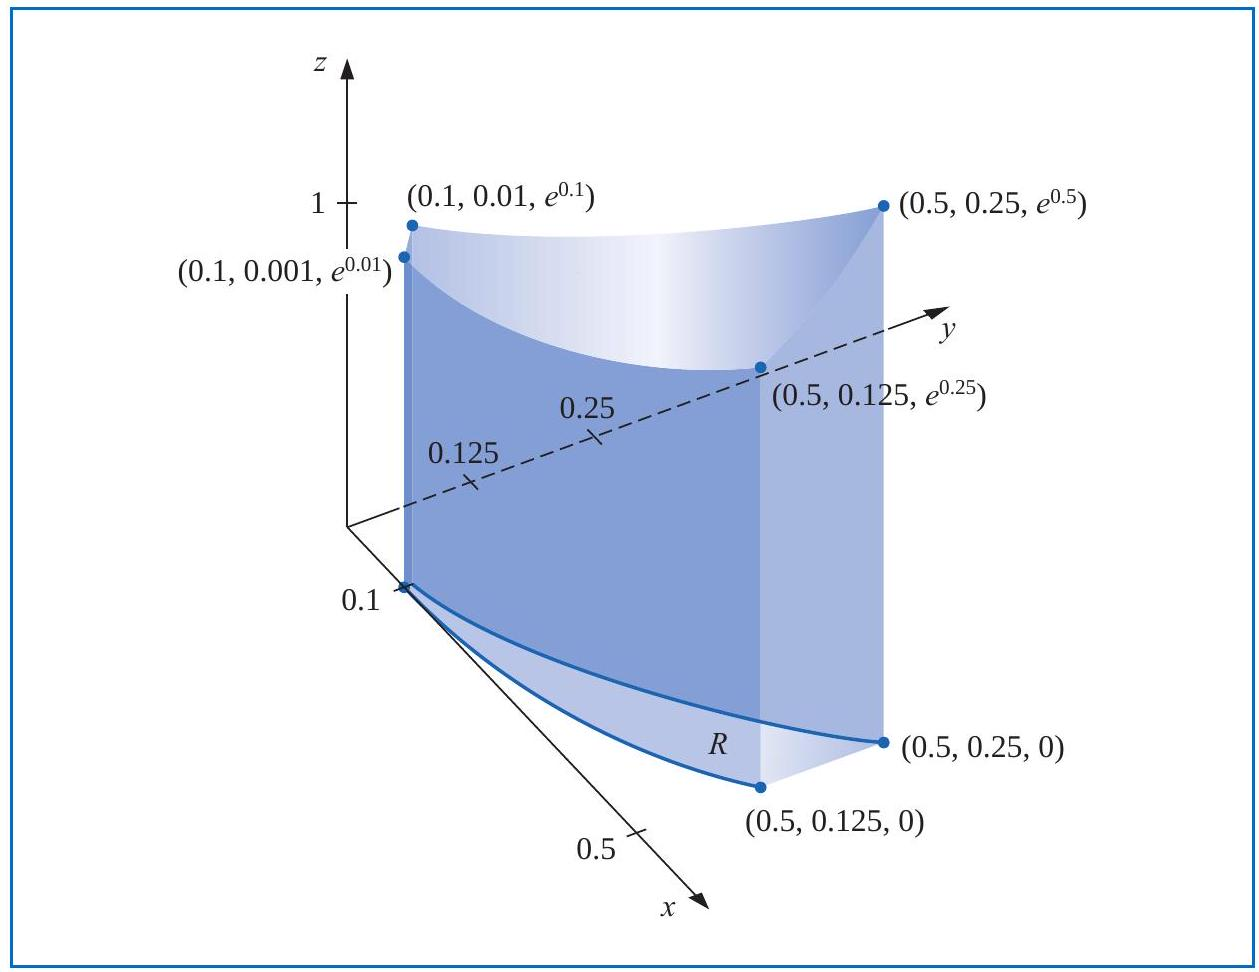
\includegraphics[width=10cm]{2025_05_15_85b7f7df47271a498e1dg-72(1)}
\caption{\scriptsize Figure $4$}
\label{fig:multipleintegralill1}
\end{figure}
%
%The reduced calculation makes it almost always worthwhile to apply Gaussian quadrature rather than a Simpson's technique when approximating triple or higher integrals.
%
\subsection*{Triple Integral Approximation}
Triple integrals of the form

$$
\int_{a}^{b} \int_{c(x)}^{d(x)} \int_{\alpha(x, y)}^{\beta(x, y)} f(x, y, z) d z d y d x
$$

(see Figure \ref{fig:tripleintegrlas1}) are approximated in a similar manner. Because of the number of calculations involved, Gaussian quadrature is the method of choice. 

\begin{figure}[h]
\centering
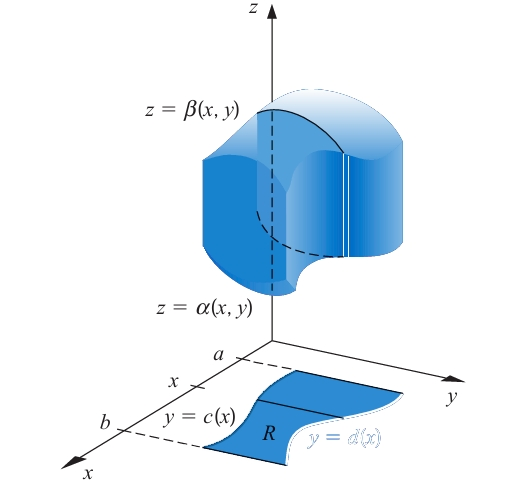
\includegraphics[width=10cm]{tripleintegrlas1}
\caption{\scriptsize Figure $5$}
\label{fig:tripleintegrlas1}
\end{figure}

%Figure 4.23
%
%\section*{Gaussian Triple Integral}
%To approximate the integral
%
%$$
%\int_{a}^{b} \int_{c(x)}^{d(x)} \int_{\alpha(x, y)}^{\beta(x, y)} f(x, y, z) d z d y d x
%$$
%
%INPUT endpoints $a, b$; positive integers $m, n, p$.\\
%(The roots $r_{i, j}$ and coefficients $c_{i, j}$ need to be available for $i=\max \{n, m, p\}$ and for $1 \leq j \leq i$.)
%
%\section*{OUTPUT approximation $J$ to $I$.}
%Step 1 Set $h_{1}=(b-a) / 2$;
%
%$$
%\begin{aligned}
%& h_{2}=(b+a) / 2 ; \\
%& J=0 .
%\end{aligned}
%$$
%
%Step 2 For $i=1,2, \ldots, m$ do Steps 3-8.\\
%\includegraphics[max width=\textwidth, center]{2025_05_15_85b7f7df47271a498e1dg-74}
%
%Step 3 Set $J X=0$;
%
%$$
%\begin{aligned}
%& x=h_{1} r_{m, i}+h_{2} ; \\
%& d_{1}=d(x) ; \\
%& c_{1}=c(x) ; \\
%& k_{1}=\left(d_{1}-c_{1}\right) / 2 ; \\
%& k_{2}=\left(d_{1}+c_{1}\right) / 2 .
%\end{aligned}
%$$
%
%Step 4 For $j=1,2, \ldots, n$ do Steps 5-7.\\
%Step 5 Set $J Y=0$;
%
%$$
%\begin{aligned}
%& y=k_{1} r_{n, j}+k_{2} ; \\
%& \beta_{1}=\beta(x, y) ; \\
%& \alpha_{1}=\alpha(x, y) ; \\
%& l_{1}=\left(\beta_{1}-\alpha_{1}\right) / 2 ; \\
%& l_{2}=\left(\beta_{1}+\alpha_{1}\right) / 2 .
%\end{aligned}
%$$
%
%Step 6 For $k=1,2, \ldots, p$ do
%
%$$
%\begin{aligned}
%& \text { set } z=l_{1} r_{p, k}+l_{2} \\
%& \quad Q=f(x, y, z) \\
%& \quad J Y=J Y+c_{p, k} Q
%\end{aligned}
%$$
%
%Step $7 \quad$ Set $J X=J X+c_{n, j} l_{1} J Y$.\\
%Step $8 \quad$ Set $J=J+c_{m, i} k_{1} J X$.\\
%Step 9 Set $J=h_{1} J$.\\
%Step 10 OUTPUT (J);\\
%STOP.
%
The following example requires the evaluation of four triple integrals.

\begin{example}
The center of a mass of a solid region $D$ with density function $\sigma$ occurs at

$$
(\bar{x}, \bar{y}, \bar{z})=\left(\frac{M_{y z}}{M}, \frac{M_{x z}}{M}, \frac{M_{x y}}{M}\right),
$$

where

$$
M_{y z}=\iiint_{D} x \sigma(x, y, z) d V, \quad M_{x z}=\iiint_{D} y \sigma(x, y, z) d V
$$

and

$$
M_{x y}=\iiint_{D} z \sigma(x, y, z) d V
$$

are the moments about the coordinate planes and the mass of $D$ is

$$
M=\iiint_{D} \sigma(x, y, z) d V
$$

The solid shown in Figure \ref{fig:tripitegillus2} is bounded by the upper nappe of the cone $z^{2}=x^{2}+y^{2}$ and the plane $z=2$. Suppose that this solid has density function given by

$$
\sigma(x, y, z)=\sqrt{x^{2}+y^{2}}
$$


Applying the Gaussian Triple Integral procedure with $n=m=p=5$ requires 125 function evaluations per integral and gives the following approximations:

$$
\begin{aligned}
M & =\int_{-2}^{2} \int_{-\sqrt{4-x^{2}}}^{\sqrt{4-x^{2}}} \int_{\sqrt{x^{2}+y^{2}}}^{2} \sqrt{x^{2}+y^{2}} d z d y d x \\
& =4 \int_{0}^{2} \int_{0}^{\sqrt{4-x^{2}}} \int_{\sqrt{x^{2}+y^{2}}}^{2} \sqrt{x^{2}+y^{2}} d z d y d x \approx 8.37504476 \\
M_{y z} & =\int_{-2}^{2} \int_{-\sqrt{4-x^{2}}}^{\sqrt{4-x^{2}}} \int_{\sqrt{x^{2}+y^{2}}}^{2} x \sqrt{x^{2}+y^{2}} d z d y d x \approx-5.55111512 \times 10^{-17} \\
M_{x z} & =\int_{-2}^{2} \int_{-\sqrt{4-x^{2}}}^{\sqrt{4-x^{2}}} \int_{\sqrt{x^{2}+y^{2}}}^{2} y \sqrt{x^{2}+y^{2}} d z d y d x \approx-8.01513675 \times 10^{-17} \\
M_{x y} & =\int_{-2}^{2} \int_{-\sqrt{4-x^{2}}}^{\sqrt{4-x^{2}}} \int_{\sqrt{x^{2}+y^{2}}}^{2} z \sqrt{x^{2}+y^{2}} d z d y d x \approx 13.40038156
\end{aligned}
$$

This implies that the approximate location of the center of mass is

$$
(\bar{x}, \bar{y}, \bar{z})=(0,0,1.60003701)
$$

These integrals are quite easy to evaluate directly. If you do this, you will find that the exact center of mass occurs at $(0,0,1.6)$.
\end{example}

%Figure 4.24\\
\begin{figure}[h]
\centering
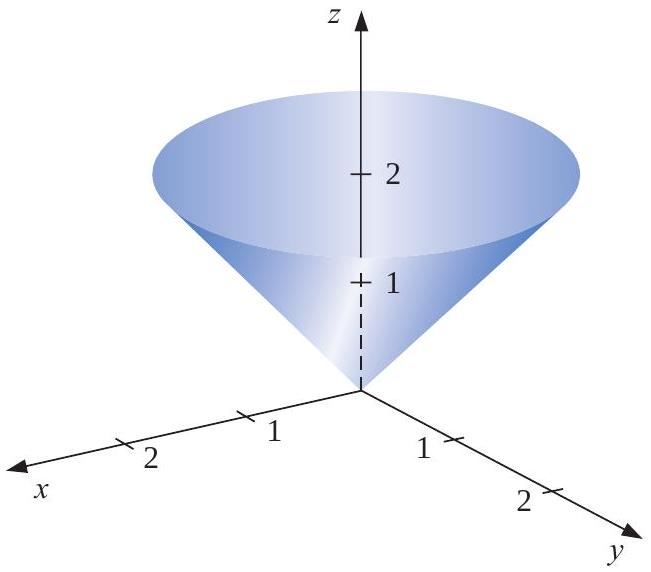
\includegraphics[width=8cm]{2025_05_15_85b7f7df47271a498e1dg-75}
\caption{\scriptsize Figure $6$ }
\label{fig:tripitegillus2}
\end{figure}
%


%Multiple integrals can be evaluated in Maple using the MultInt command in the MultivariateCalculus subpackage of the Student package. For example, to evaluate the multiple integral
%
%$$
%\int_{2}^{4} \int_{x-1}^{x+6} \int_{-2}^{4+y^{2}} x^{2}+y^{2}+z d z d y d x
%$$
%
%we first load the package and define the function with\\[0pt]
%with(Student[MultivariateCalculus]): $f:=(x, y, z) \rightarrow x^{2}+y^{2}+z$\\
%Then issue the command\\
%MultiInt $\left(f(x, y, z), z=-2 . .4+y^{2}, y=x-1 . . x+6, x=2 . .4\right)$\\
%which produces the result\\
%1.995885970

\begin{myexercise}%\label{Comprehensionquiz2}
Consider the following algorithm

\begin{boxB}Algorithm: Simpson's Double Integral\\
To approximate the integral

$$
I=\int_{a}^{b} \int_{c(x)}^{d(x)} f(x, y) d y d x
$$

INPUT endpoints $a, b$ : even positive integers $m, n$.\\
OUTPUT approximation $J$ to $I$.\\
Step 1 Set $h=(b-a) / n$;\\
\hspace*{2cm}$J_{1}=0 ; \quad($ End terms.$)$\\
\hspace*{2cm}$J_{2}=0 ; \quad$ (Even terms.)\\
\hspace*{2cm}$J_{3}=0 . \quad$ (Odd terms.)\\
Step 2 For $i=0,1, \ldots, n$ do Steps 3-8.\\
\hspace*{1cm}Step 3 Set $x=a+i h$; (Composite Simpson's method for $x$.)

$$
\begin{aligned}
& H X=(d(x)-c(x)) / m ; \\
& K_{1}=f(x, c(x))+f(x, d(x)) ; \quad(\text { End terms } .) \\
& K_{2}=0 ; \quad(\text { Even terms } .) \\
& K_{3}=0 . \quad(\text { Odd terms } .)
\end{aligned}
$$

\hspace*{1cm}Step 4 For $j=1,2, \ldots, m-1$ do Step 5 and 6.\\
\hspace*{2.5cm}Step 5 Set $y=c(x)+j H X$;

$$
Q=f(x, y)
$$

\hspace*{2.5cm}Step 6 If $j$ is even then set $K_{2}=K_{2}+Q$\\
\hspace*{4cm} else set $K_{3}=K_{3}+Q$.

Step 7 Set $L=\left(K_{1}+2 K_{2}+4 K_{3}\right) H X / 3$.\\
$\left(L \approx \int_{c\left(x_{i}\right)}^{d\left(x_{i}\right)} f\left(x_{i}, y\right) d y\right.$ by the Composite Simpson's method.)\\
Step 8 If $i=0$ or $i=n$ then set $J_{1}=J_{1}+L$\\
\hspace*{3cm} else if $i$ is even then set $J_{2}=J_{2}+L$ \\
\hspace*{3cm}else set $J_{3}=J_{3}+L$.

%The reduced calculation makes it generally worthwhile to apply\\
%Gaussian quadrature rather than a Simpson's technique when approximating double integrals.

Step 9 Set $J=h\left(J_{1}+2 J_{2}+4 J_{3}\right) / 3$.\\
Step 10 OUTPUT (J); STOP.
\end{boxB}
Use this algorithm with $n=m=4$ to approximate the following double integrals, and compare the results to the exact answers.
\begin{multicols}{2}
\begin{enumerate}[label=(\alph*)]
\item $\int_{2.1}^{2.5} \int_{1.2}^{1.4} x y^{2} d y d x$\\
\item $\int_{0}^{0.5} \int_{0}^{0.5} e^{y-x} d y d x$
\item $\int_{2}^{2.2} \int_{x}^{2 x}\left(x^{2}+y^{3}\right) d y d x$\\
\item $\int_{1}^{1.5} \int_{0}^{x}\left(x^{2}+\sqrt{y}\right) d y d x$
 \end{enumerate}
\end{multicols}
\end{myexercise}

\begin{mysolution}
\begin{multicols}{4}
\begin{enumerate}[label=(\alph*)]
\item $0.3115733$
\item $0.2552526$
\item $16.50864$
\item $1.476684$
 \end{enumerate}
\end{multicols}
\end{mysolution}

\section{Improper Integrals}
\videolesson
\begin{selfvideo}[2]
%LESSON 3: 
This video presents a discussion on numerical methods for improper integrals. Follow the discussion and then solve the problems in the subsequent quiz.
\end{selfvideo}

Improper integrals result when the notion of integration is extended either to an interval of integration on which the function is unbounded or to an interval with one or more infinite endpoints. In either circumstance, the normal rules of integral approximation must be modified.

\subsection*{Left Endpoint Singularity}
We will first consider the situation when the integrand is unbounded at the left endpoint of the interval of integration, as shown in Figure \ref{fig:imprpint1}. In this case we say that $f$ has a singularity at the endpoint $a$. We will then show how other improper integrals can be reduced to problems of this form.

%Figure 4.25\\
\begin{figure}
\centering
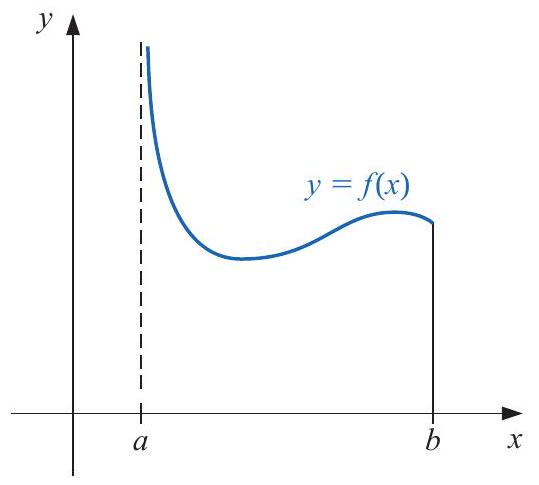
\includegraphics[width=8cm]{2025_05_15_85b7f7df47271a498e1dg-78}
\caption{\scriptsize Figure $7$}
\label{fig:imprpint1}
\end{figure}

It is shown in calculus that the improper integral with a singularity at the left endpoint,

$$
\int_{a}^{b} \frac{d x}{(x-a)^{p}}
$$

converges if and only if $0<p<1$, and in this case, we define

$$
\int_{a}^{b} \frac{1}{(x-a)^{p}} d x=\left.\lim _{M \rightarrow a^{+}} \frac{(x-a)^{1-p}}{1-p}\right|_{x=M} ^{x=b}=\frac{(b-a)^{1-p}}{1-p}
$$

\begin{example}
Show that the improper integral $\int_{0}^{1} \frac{1}{\sqrt{x}} d x$ converges but $\int_{0}^{1} \frac{1}{x^{2}} d x$ diverges.
\end{example}

\begin{mysolution}
For the first integral we have

$$
\int_{0}^{1} \frac{1}{\sqrt{x}} d x=\lim _{M \rightarrow 0^{+}} \int_{M}^{1} x^{-1 / 2} d x=\left.\lim _{M \rightarrow 0^{+}} 2 x^{1 / 2}\right|_{x=M} ^{x=1}=2-0=2
$$

but the second integral

$$
\int_{0}^{1} \frac{1}{x^{2}} d x=\lim _{M \rightarrow 0^{+}} \int_{M}^{1} x^{-2} d x=\lim _{M \rightarrow 0^{+}}-\left.x^{-1}\right|_{x=M} ^{x=1}
$$

is unbounded.

If $f$ is a function that can be written in the form

$$
f(x)=\frac{g(x)}{(x-a)^{p}}
$$

where $0<p<1$ and $g$ is continuous on $[a, b]$, then the improper integral

$$
\int_{a}^{b} f(x) d x
$$

also exists. We will approximate this integral using the Composite Simpson's rule, provided that $g \in C^{5}[a, b]$. In that case, we can construct the fourth Taylor polynomial, $P_{4}(x)$, for $g$ about $a$,

$$
P_{4}(x)=g(a)+g^{\prime}(a)(x-a)+\frac{g^{\prime \prime}(a)}{2!}(x-a)^{2}+\frac{g^{\prime \prime \prime}(a)}{3!}(x-a)^{3}+\frac{g^{(4)}(a)}{4!}(x-a)^{4},
$$

and write


\begin{equation}\label{eqn:impropinteeaxm1eqn1}
\int_{a}^{b} f(x) d x=\int_{a}^{b} \frac{g(x)-P_{4}(x)}{(x-a)^{p}} d x+\int_{a}^{b} \frac{P_{4}(x)}{(x-a)^{p}} d x 
\end{equation}


Because $P(x)$ is a polynomial, we can exactly determine the value of


\begin{equation}\label{eqn:impropinteeaxm1eqn2}
\int_{a}^{b} \frac{P_{4}(x)}{(x-a)^{p}} d x=\sum_{k=0}^{4} \int_{a}^{b} \frac{g^{(k)}(a)}{k!}(x-a)^{k-p} d x=\sum_{k=0}^{4} \frac{g^{(k)}(a)}{k!(k+1-p)}(b-a)^{k+1-p}
\end{equation}


This is generally the dominant portion of the approximation, especially when the Taylor polynomial $P_{4}(x)$ agrees closely with $g(x)$ throughout the interval $[a, b]$.

To approximate the integral of $f$, we must add to this value the approximation of

$$
\int_{a}^{b} \frac{g(x)-P_{4}(x)}{(x-a)^{p}} d x
$$

To determine this, we first define

$$
G(x)= \begin{cases}\frac{g(x)-P_{4}(x)}{(x-a)^{p}}, & \text { if } a<x \leq b, \\ 0, & \text { if } x=a .\end{cases}
$$
\end{mysolution}
This gives us a continuous function on $[a, b]$. In fact, $0<p<1$ and $P_{4}^{(k)}(a)$ agrees with $g^{(k)}(a)$ for each $k=0,1,2,3,4$, so we have $G \in C^{4}[a, b]$. This implies that the Composite Simpson's rule can be applied to approximate the integral of $G$ on $[a, b]$. Adding this approximation to the value in Eq. \ref{eqn:impropinteeaxm1eqn2} gives an approximation to the improper integral of $f$ on $[a, b]$, within the accuracy of the Composite Simpson's rule approximation.

\begin{example}
Use Composite Simpson's rule with $h=0.25$ to approximate the value of the improper integral

$$
\int_{0}^{1} \frac{e^{x}}{\sqrt{x}} d x
$$
\end{example}

\begin{mysolution}
The fourth Taylor polynomial for $e^{x}$ about $x=0$ is

$$
P_{4}(x)=1+x+\frac{x^{2}}{2}+\frac{x^{3}}{6}+\frac{x^{4}}{24},
$$

so the dominant portion of the approximation to $\int_{0}^{1} \frac{e^{x}}{\sqrt{x}} d x$ is

$$
\begin{aligned}
\int_{0}^{1} \frac{P_{4}(x)}{\sqrt{x}} d x & =\int_{0}^{1}\left(x^{-1 / 2}+x^{1 / 2}+\frac{1}{2} x^{3 / 2}+\frac{1}{6} x^{5 / 2}+\frac{1}{24} x^{7 / 2}\right) d x \\
& =\lim _{M \rightarrow 0^{+}}\left[2 x^{1 / 2}+\frac{2}{3} x^{3 / 2}+\frac{1}{5} x^{5 / 2}+\frac{1}{21} x^{7 / 2}+\frac{1}{108} x^{9 / 2}\right]_{M}^{1} \\
& =2+\frac{2}{3}+\frac{1}{5}+\frac{1}{21}+\frac{1}{108} \approx 2.9235450
\end{aligned}
$$

For the second portion of the approximation to $\int_{0}^{1} \frac{e^{x}}{\sqrt{x}} d x$ we need to approximate $\int_{0}^{1} G(x) d x$, where

$$
G(x)= \begin{cases}\frac{1}{\sqrt{x}}\left(e^{x}-P_{4}(x)\right), & \text { if } 0<x \leq 1 \\ 0, & \text { if } x=0\end{cases}
$$



Table \ref{tab:impropinteexam1} lists the values needed for the Composite Simpson's rule for this approximation.\\
Using these data and the Composite Simpson's rule gives

$$
\begin{aligned}
\int_{0}^{1} G(x) d x & \approx \frac{0.25}{3}[0+4(0.0000170)+2(0.0004013)+4(0.0026026)+0.0099485] \\
& =0.0017691
\end{aligned}
$$

Hence

$$
\int_{0}^{1} \frac{e^{x}}{\sqrt{x}} d x \approx 2.9235450+0.0017691=2.9253141
$$

This result is accurate to within the accuracy of the Composite Simpson's rule approximation for the function $G$. Because $\left|G^{(4)}(x)\right|<1$ on $[0,1]$, the error is bounded by

$$
\frac{1-0}{180}(0.25)^{4}=0.0000217
$$\qed
\end{mysolution}
%Table 4.13

\begin{table}[h]
\centering
\begin{tabular}{cl}
\hline
$x$ & \multicolumn{1}{c}{$G(x)$} \\
\hline
0.00 & 0 \\
0.25 & 0.0000170 \\
0.50 & 0.0004013 \\
0.75 & 0.0026026 \\
1.00 & 0.0099485 \\
\hline
\end{tabular}
\caption{}
\label{tab:impropinteexam1}
\end{table}


\subsection*{Right Endpoint Singularity}
To approximate the improper integral with a singularity at the right endpoint, we could develop a similar technique but expand in terms of the right endpoint $b$ instead of the left endpoint $a$. Alternatively, we can make the substitution

$$
z=-x, \quad d z=-d x
$$

to change the improper integral into one of the form


\begin{equation*}
\int_{a}^{b} f(x) d x=\int_{-b}^{-a} f(-z) d z \tag{4.46}
\end{equation*}


which has its singularity at the left endpoint. Then we can apply the left endpoint singularity technique we have already developed. (See Figure \ref{fig:impropintrightep}.)

%Figure 4.26\\
\begin{figure}
\centering
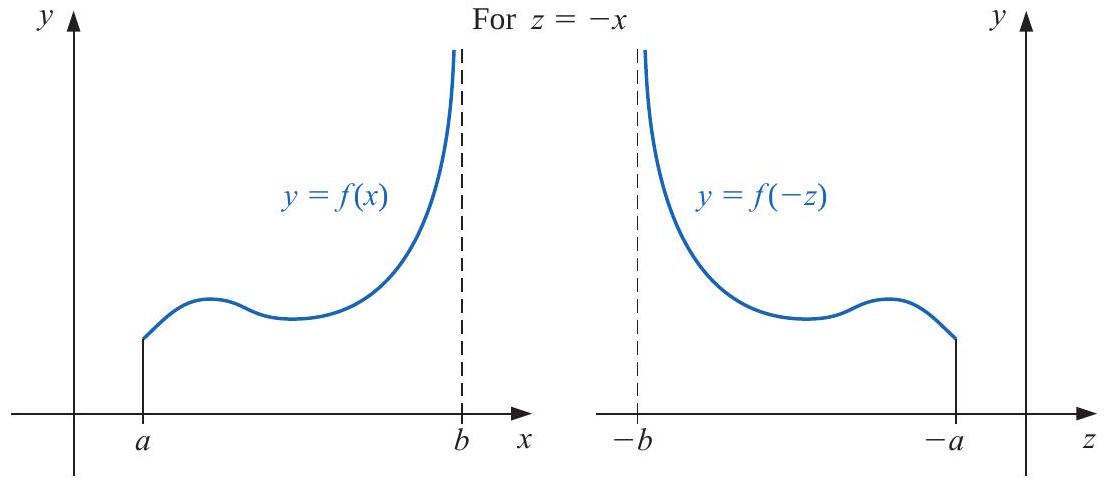
\includegraphics[width=10cm]{2025_05_15_85b7f7df47271a498e1dg-81}
\caption{\scriptsize Figure $8$}
\label{fig:impropintrightep}
\end{figure}

An improper integral with a singularity at $c$, where $a<c<b$, is treated as the sum of improper integrals with endpoint singularities since

$$
\int_{a}^{b} f(x) d x=\int_{a}^{c} f(x) d x+\int_{c}^{b} f(x) d x
$$

\subsection*{Infinite Singularity}
The other type of improper integral involves infinite limits of integration. The basic integral of this type has the form

$$
\int_{a}^{\infty} \frac{1}{x^{p}} d x
$$

for $p>1$. This is converted to an integral with left endpoint singularity at 0 by making the integration substitution

$$
t=x^{-1}, \quad d t=-x^{-2} d x, \quad \text { so } \quad d x=-x^{2} d t=-t^{-2} d t .
$$

Then

$$
\int_{a}^{\infty} \frac{1}{x^{p}} d x=\int_{1 / a}^{0}-\frac{t^{p}}{t^{2}} d t=\int_{0}^{1 / a} \frac{1}{t^{2-p}} d t
$$

In a similar manner, the variable change $t=x^{-1}$ converts the improper integral $\int_{a}^{\infty} f(x) d x$ into one that has a left endpoint singularity at zero:


\begin{equation}\label{eqn:infising}
\int_{a}^{\infty} f(x) d x=\int_{0}^{1 / a} t^{-2} f\left(\frac{1}{t}\right) d t
\end{equation}


It can now be approximated using a quadrature formula of the type described earlier.

\begin{example}
Approximate the value of the improper integral

$$
I=\int_{1}^{\infty} x^{-3 / 2} \sin \frac{1}{x} d x
$$
\end{example}

\begin{mysolution}
We first make the variable change $t=x^{-1}$, which converts the infinite singularity into one with a left endpoint singularity. Then

$$
d t=-x^{-2} d x, \quad \text { so } \quad d x=-x^{2} d t=-\frac{1}{t^{2}} d t
$$

and

$$
I=\int_{x=1}^{x=\infty} x^{-3 / 2} \sin \frac{1}{x} d x=\int_{t=1}^{t=0}\left(\frac{1}{t}\right)^{-3 / 2} \sin t\left(-\frac{1}{t^{2}} d t\right)=\int_{0}^{1} t^{-1 / 2} \sin t d t
$$

The fourth Taylor polynomial, $P_{4}(t)$, for $\sin t$ about 0 is

$$
P_{4}(t)=t-\frac{1}{6} t^{3}
$$

so

$$
G(t)= \begin{cases}\frac{\sin t-t+\frac{1}{6} t^{3}}{t^{1 / 2}}, & \text { if } 0<t \leq 1 \\ 0, & \text { if } t=0\end{cases}
$$

is in $C^{4}[0,1]$, and we have

$$
\begin{aligned}
I & =\int_{0}^{1} t^{-1 / 2}\left(t-\frac{1}{6} t^{3}\right) d t+\int_{0}^{1} \frac{\sin t-t+\frac{1}{6} t^{3}}{t^{1 / 2}} d t \\
& =\left[\frac{2}{3} t^{3 / 2}-\frac{1}{21} t^{7 / 2}\right]_{0}^{1}+\int_{0}^{1} \frac{\sin t-t+\frac{1}{6} t^{3}}{t^{1 / 2}} d t \\
& =0.61904761+\int_{0}^{1} \frac{\sin t-t+\frac{1}{6} t^{3}}{t^{1 / 2}} d t
\end{aligned}
$$

The result from the Composite Simpson's rule with $n=16$ for the remaining integral is 0.0014890097 . This gives a final approximation of

$$
I=0.0014890097+0.61904761=0.62053661
$$

which is accurate to within $4.0 \times 10^{-8}$.
\end{mysolution}
\begin{myexercise}%\label{Comprehensionquiz2}
Use Simpson's Composite rule and the given values of $n$ to approximate the following improper integrals.
\begin{multicols}{2}
\begin{enumerate}[label=(\alph*)]
\item $\int_{0}^{1} x^{-1 / 4} \sin x d x, \quad n=4$\\
\item $\int_{0}^{1} \frac{e^{2 x}}{\sqrt[5]{x^{2}}} d x, \quad n=6$
\item $\quad \int_{1}^{2} \frac{\ln x}{(x-1)^{1 / 5}} d x, \quad n=8$\\
\item $\quad \int_{0}^{1} \frac{\cos 2 x}{x^{1 / 3}} d x, \quad n=6$
\end{enumerate}
\end{multicols}

\begin{mysolution}
The Composite Simpson’s rule gives:
\begin{multicols}{2}
\begin{enumerate}[label=(\alph*)]
\item $0.5284163$
\item $4.266654$
\item $0.4329748$
\item $0.8802210$
\end{enumerate}
\end{multicols}
\end{mysolution}
\end{myexercise}



\section{The Elementary Theory of Initial-Value Problems}
%\activities
%Read on the elementary theory of initial-value problems in pages \textcolor{red}{\bf page $260-264$} of the following reference and then attempt the subsequent quiz
%\begin{activity}[\cg Reading]
%\begin{enumerate}
%\item Burden, R. L., Faires, J. D., Burden, A. M. (2015). Numerical Analysis. Tenth Edition, Cengage Learning.\\
%\end{enumerate}
%\end{activity}
\videolesson
\begin{selfvideo}[2]
%LESSON 3: 
This video presents a discussion on the elementary theory of initial-value problems. Follow the discussion and then solve the problems in the subsequent quiz.
\end{selfvideo}
Differential equations are used to model problems in science and engineering that involve the change of some variable with respect to another. Most of these problems require the solution to a differential equation that satisfies a given initial condition.

In common real-life situations, the differential equation that models the problem is too complicated to solve exactly. One approach in solving such equations uses methods for approximating the solution of the original problem. This approach is most commonly taken because the approximation methods give more accurate results and realistic error information.

The methods that we consider here give approximations found at certain specified, and often equally spaced, points.

We need some definitions and results from the theory of ordinary differential equations before considering methods for approximating the solutions to initial-value problems.

\begin{definition}
A function $f(t, y)$ is said to satisfy a Lipschitz condition in the variable $y$ on a set $D \subset \mathbb{R}^{2}$ if a constant $L>0$ exists with

$$
\left|f\left(t, y_{1}\right)-f\left(t, y_{2},\right)\right| \leq L\left|y_{1}-y_{2}\right|
$$

whenever $\left(t, y_{1}\right)$ and $\left(t, y_{2}\right)$ are in $D$. The constant $L$ is called a {\bf Lipschitz constant} for $f$.
\end{definition}

\begin{example}
Show that $f(t, y)=t|y|$ satisfies a Lipschitz condition on the interval $D=\{(t, y) \mid 1 \leq$ $t \leq 2$ and $-3 \leq y \leq 4\}$.
\end{example}

\begin{mysolution}
For each pair of points $\left(t, y_{1}\right)$ and $\left(t, y_{2}\right)$ in $D$ we have

$$
\left|f\left(t, y_{1}\right)-f\left(t, y_{2}\right)\right|=|t| y_{1}|-t| y_{2}\|=|t|\| y_{1}\left|-\left|y_{2} \| \leq 2\right| y_{1}-y_{2}\right|
$$

Thus $f$ satisfies a Lipschitz condition on $D$ in the variable $y$ with Lipschitz constant 2 . The smallest value possible for the Lipschitz constant for this problem is $L=2$, because, for example,

$$
|f(2,1)-f(2,0)|=|2-0|=2|1-0|
$$
\end{mysolution}

\begin{definition}\label{def:convex}
A set $D \subset \mathbb{R}^{2}$ is said to be convex if whenever $\left(t_{1}, y_{1}\right)$ and $\left(t_{2}, y_{2}\right)$ belong to $D$, then $\left((1-\lambda) t_{1}+\lambda t_{2},(1-\lambda) y_{1}+\lambda y_{2}\right)$ also belongs to $D$ for every $\lambda$ in $[0,1]$.
\end{definition}

In geometric terms, Definition \ref{def:convex} states that a set is convex provided that whenever two points belong to the set, the entire straight-line segment between the points also belongs to the set. (See Figure \ref{fig:convex1}.) The sets we consider in this chapter are generally of the form $D=\{(t, y) \mid a \leq t \leq b$ and $-\infty<y<\infty\}$ for some constants $a$ and $b$. It is easy to verify that these sets are convex.
%
%Figure 5.1\\
\begin{figure}[h]
\centering
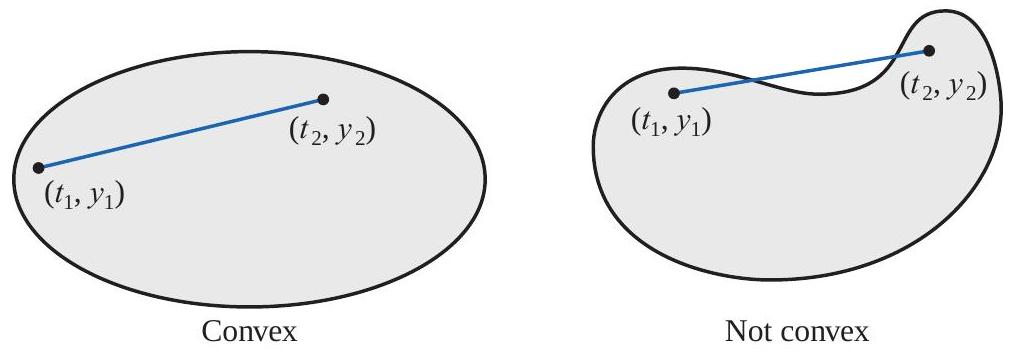
\includegraphics[width=10cm]{2025_05_15_5266fa2c85d567bd073dg-03}
\caption{\scriptsize Figure $10$}
\label{fig:convex1}
\end{figure}

\begin{theorem}\label{thm:elementarytheofIVPtm1}
Suppose $f(t, y)$ is defined on a convex set $D \subset \mathbb{R}^{2}$. If a constant $L>0$ exists with

%Rudolf Lipschitz (1832-1903) worked in many branches of mathematics, including number theory, Fourier series, differential equations, analytical mechanics, and potential theory. He is best known for this generalization of the work of Augustin-Louis Cauchy (1789-1857) and Guiseppe Peano (1856-1932).


\begin{equation}\label{eqn:elementarytheofIVPeq1}
\left|\frac{\partial f}{\partial y}(t, y)\right| \leq L, \quad \text { for all }(t, y) \in D,
\end{equation}


then $f$ satisfies a Lipschitz condition on $D$ in the variable $y$ with Lipschitz constant $L$.
\end{theorem}


As the next theorem will show, it is often of significant interest to determine whether the function involved in an initial-value problem satisfies a Lipschitz condition in its second\\
variable, and condition \ref{eqn:elementarytheofIVPeq1} is generally easier to apply than the definition. We should note, however, that Theorem $1$ gives only sufficient conditions for a Lipschitz condition to hold. The function in Example 1, for instance, satisfies a Lipschitz condition, but the partial derivative with respect to $y$ does not exist when $y=0$.

%The following theorem is a version of the fundamental existence and uniqueness theorem for first-order ordinary differential equations. 

\begin{theorem}\label{thm:elementarytheofIVPtm2}
Suppose that $D=\{(t, y) \mid a \leq t \leq b$ and $-\infty<y<\infty\}$ and that $f(t, y)$ is continuous on $D$. If $f$ satisfies a Lipschitz condition on $D$ in the variable $y$, then the initial-value problem

$$
y^{\prime}(t)=f(t, y), \quad a \leq t \leq b, \quad y(a)=\alpha,
$$

has a unique solution $y(t)$ for $a \leq t \leq b$.
\end{theorem}

\begin{example}
Use Theorem $2$ to show that there is a unique solution to the initial-value problem

$$
y^{\prime}=1+t \sin (t y), \quad 0 \leq t \leq 2, \quad y(0)=0 .
$$
\end{example}

\begin{mysolution}
Holding $t$ constant and applying the Mean Value Theorem to the function

$$
f(t, y)=1+t \sin (t y)
$$

we find that when $y_{1}<y_{2}$, a number $\xi$ in ( $y_{1}, y_{2}$ ) exists with

$$
\frac{f\left(t, y_{2}\right)-f\left(t, y_{1}\right)}{y_{2}-y_{1}}=\frac{\partial}{\partial y} f(t, \xi)=t^{2} \cos (\xi t)
$$

Thus

$$
\left|f\left(t, y_{2}\right)-f\left(t, y_{1}\right)\right|=\left|y_{2}-y_{1}\right|\left|t^{2} \cos (\xi t)\right| \leq 4\left|y_{2}-y_{1}\right|
$$

and $f$ satisfies a Lipschitz condition in the variable $y$ with Lipschitz constant $L=4$. Additionally, $f(t, y)$ is continuous when $0 \leq t \leq 2$ and $-\infty<y<\infty$, so Theorem $2$ implies that a unique solution exists to this initial-value problem.\qed
\end{mysolution}

%If you have completed a course in differential equations you might try to find the exact solution to this problem.
%
\subsection*{Well-Posed Problems}
%Now that we have, to some extent, taken care of the question of when initial-value problems have unique solutions, we can move to the second important consideration when approximating the solution to an initial-value problem. Initial-value problems obtained by observing physical phenomena generally only approximate the true situation, so we need to know whether small changes in the statement of the problem introduce correspondingly small changes in the solution. This is also important because of the introduction of round-off error when numerical methods are used. That is,

\begin{boxB}
\underline{Question:} How do we determine whether a particular problem has the property that small changes, or perturbations, in the statement of the problem introduce correspondingly small changes in the solution?
\end{boxB}

First consider the following workable definition to express this concept.

\begin{definition} 
The initial-value problem

\begin{equation}\label{eqn:wellpossedeq1}
\frac{d y}{d t}=f(t, y), \quad a \leq t \leq b, \quad y(a)=\alpha,
\end{equation}

is said to be a well-posed problem if:

\begin{itemize}
  \item A unique solution, $y(t)$, to the problem exists, and
  \item There exist constants $\varepsilon_{0}>0$ and $k>0$ such that for any $\varepsilon$, with $\varepsilon_{0}>\varepsilon>0$, whenever $\delta(t)$ is continuous with $|\delta(t)|<\varepsilon$ for all $t$ in $[a, b]$, and when $\left|\delta_{0}\right|<\varepsilon$, the initial-value problem


\begin{equation}\label{eqn:wellpossedeq2}
\frac{d z}{d t}=f(t, z)+\delta(t), \quad a \leq t \leq b, \quad z(a)=\alpha+\delta_{0}
\end{equation}

has a unique solution $z(t)$ that satisfies

$$
|z(t)-y(t)|<k \varepsilon \quad \text { for all } t \text { in }[a, b]
$$
\end{itemize}
\end{definition}
The problem specified by \ref{eqn:wellpossedeq2} is called a {\bf perturbed problem} associated with the original problem \ref{eqn:wellpossedeq1}. It assumes the possibility of an error being introduced in the statement of the differential equation, as well as an error $\delta_{0}$ being present in the initial condition.

%Numerical methods will always be concerned with solving a perturbed problem because any round-off error introduced in the representation perturbs the original problem. Unless the original problem is well-posed, there is little reason to expect that the numerical solution to a perturbed problem will accurately approximate the solution to the original problem.

The following theorem specifies conditions that ensure that an initial-value problem is well-posed.

\begin{theorem}\label{thm:wellposedcond}
Suppose $D=\{(t, y) \mid a \leq t \leq b$ and $-\infty<y<\infty\}$. If $f$ is continuous and satisfies a Lipschitz condition in the variable $y$ on the set $D$, then the initial-value problem

$$
\frac{d y}{d t}=f(t, y), \quad a \leq t \leq b, \quad y(a)=\alpha
$$

is well-posed.
\end{theorem}

\begin{example}
Show that the initial-value problem

\begin{equation}\label{eqn:ivpeam3eq}
\frac{d y}{d t}=y-t^{2}+1, \quad 0 \leq t \leq 2, \quad y(0)=0.5
\end{equation}


is well posed on $D=\{(t, y) \mid 0 \leq t \leq 2$ and $-\infty<y<\infty\}$.
\end{example}

\begin{mysolution}
Because

$$
\left|\frac{\partial\left(y-t^{2}+1\right)}{\partial y}\right|=|1|=1
$$

Theorem $1$ implies that $f(t, y)=y-t^{2}+1$ satisfies a Lipschitz condition in $y$ on $D$ with Lipschitz constant $1$. Since $f$ is continuous on $D$, Theorem $3$ implies that the problem is well-posed.

As an illustration, consider the solution to the perturbed problem


\begin{equation}\label{eqn:ivpeam3eq1}
\frac{d z}{d t}=z-t^{2}+1+\delta, \quad 0 \leq t \leq 2, \quad z(0)=0.5+\delta_{0}
\end{equation}

%%Maple reserves the letter $D$ to represent differentiation.\\
where $\delta$ and $\delta_{0}$ are constants. The solutions to Eqs. \ref{} and \ref{} are

$$
y(t)=(t+1)^{2}-0.5 e^{t} \quad \text { and } \quad z(t)=(t+1)^{2}+\left(\delta+\delta_{0}-0.5\right) e^{t}-\delta,
$$

respectively.

Suppose that $\varepsilon$ is a positive number. If $|\delta|<\varepsilon$ and $\left|\delta_{0}\right|<\varepsilon$, then

$$
|y(t)-z(t)|=\left|\left(\delta+\delta_{0}\right) e^{t}-\delta\right| \leq\left|\delta+\delta_{0}\right| e^{2}+|\delta| \leq\left(2 e^{2}+1\right) \varepsilon
$$

for all $t$. This implies that problem \ref{} is well-posed with $k(\varepsilon)=2 e^{2}+1$ for all $\varepsilon>0$.
\end{mysolution}
%Maple can be used to solve many initial-value problems. Consider the problem
%
%$$
%\frac{d y}{d t}=y-t^{2}+1, \quad 0 \leq t \leq 2, \quad y(0)=0.5
%$$
%
%To define the differential equation and initial condition, enter\\
%deq $:=D(y)(t)=y(t)-t^{2}+1$; init $:=y(0)=0.5$\\
%The names deq and init have been chosen by the user. The command to solve the initial-value problems is\\
%deqsol $:=$ dsolve $(\{$ deq, init $\}, y(t))$\\
%and Maple responds with
%
%$$
%y(t)=1+t^{2}+2 t-\frac{1}{2} e^{t}
%$$
%
%To use the solution to obtain a specific value, such as $y(1.5)$, we enter\\
%$q:=\operatorname{rhs}($ deqsol $): \operatorname{evalf}(\operatorname{subs}(t=1.5, q))$\\
%which gives\\
%4.009155465
%
%The function $r h s$ (for $r$ ight $h$ and $s$ ide) is used to assign the solution of the initial-value problem to the function $q$, which we then evaluate at $t=1.5$.
%
%The function dsolve can fail if an explicit solution to the initial-value problem cannot be found. For example, for the initial-value problem given in Example 2, the command\\
%deqsol2 $:=$ dsolve $(\{D(y)(t)=1+t \cdot \sin (t \cdot y(t)), y(0)=0\}, y(t))$\\
%does not succeed because an explicit solution cannot be found. In this case a numerical method must be used.




\begin{myexercise}%\label{Comprehensionquiz2}
Use Theorem \ref{thm:elementarytheofIVPtm2} to show that each of the following initial-value problems has a unique solution, and find the solution.
\begin{enumerate}[label=(\alph*)]
\item $y^{\prime}=y \cos t, \quad 0 \leq t \leq 1, \quad y(0)=1$.\\
\item $y^{\prime}=\frac{2}{t} y+t^{2} e^{t}, \quad 1 \leq t \leq 2, \quad y(1)=0$.\\
\item $y^{\prime}=-\frac{2}{t} y+t^{2} e^{t}, \quad 1 \leq t \leq 2, \quad y(1)=\sqrt{2} e$.\\
\item $y^{\prime}=\frac{4 t^{3} y}{1+t^{4}}, \quad 0 \leq t \leq 1, \quad y(0)=1$.
\end{enumerate}

\begin{mysolution}
\begin{enumerate}[label=(\alph*)]
\item Since $f(t,y) = y\cos t$, we have $\frac{\partial f}{\partial y} (t,y) = \cos t$, and $f$ satisfies a Lipschitz condition in $y$ with $L = 1$ on
\[D=\{(t,y)|0\leq t\leq1,-\infty<y<\infty\}.\]
Also, $f$ is continuous on $D$, so there exists a unique solution, which is $y(t) = e^{\sin t}$.
\item Since $f(t,y) =\frac2t y +t^2e^t$, we have $\frac{\partial f}{\partial y} = \frac2t$, and $f$ satisfies a Lipschitz condition in $y$ with $L = 2$ on
\[D=\{(t,y)|1\leq t\leq2,-\infty<y<\infty\}.\]
 Also, $f$ is continuous on $D$, so there exists a unique solution, which is $y(t) = t^2(e^t-e)$.
\item Since $f(t,y) =-\frac2t y +t^2e^t$,we have $\frac{\partial f}{\partial y}=-\frac2t$, and $f$ satisfies a Lipschitz condition in $y$ with $L = 2$ on
\[D=\{(t,y)|1\leq t\leq2,-\infty<y<\infty\}.\]
Also, $f$ is continuous on $D$, so there exists a unique solution, which is
\[y(t) = (t^4e^t-4t^3e^t + 12t^2e^t-24te^t + 24e^t + (\sqrt{2}-9)e)/t^2.\]
\item Since $f(t,y) = \frac{4t^3y}{1 +t^4}$, we have $\frac{\partial f}{\partial y}=\frac{4t^3}{1 +t^4}$, and $f$ satisfies a Lipschitz condition in $y$ with $L = 2$ on
\[D=\{(t,y)|0\leq t\leq1,-\infty<y<\infty\}.\]
Also, $f$ is continuous on $D$, so there exists a unique solution, which is $y(t) = 1 + t^4$.
\end{enumerate}
\end{mysolution}
\end{myexercise}


\section{Euler's Method}
%\videolesson
%\begin{selfvideo}[2]
%%LESSON 3: 
%This video presents a discussion on Euler's method. Follow the discussion and then solve the problems in the subsequent quiz.
%\end{selfvideo}

\activities
Read on Euler's method in Section 8.02 of the reference whose link is provided below and then attempt the subsequent quiz
\begin{activity}[\cg Reading]
\mylink{https://math.libretexts.org/Workbench/Numerical\_Methods\_with\_Applications\_(Kaw)}
\end{activity}


%\begin{boxB}Question: \end{boxB}
\begin{myexercise}%\label{Comprehensionquiz2}
Use Euler's method to approximate the solutions for each of the following initial-value problems.
\begin{enumerate}[label=(\alph*)]
\item $y^{\prime}=t e^{3 t}-2 y, \quad 0 \leq t \leq 1, \quad y(0)=0$, with $h=0.5$
\item $y^{\prime}=1+(t-y)^{2}, \quad 2 \leq t \leq 3, \quad y(2)=1$, with $h=0.5$
\item $y^{\prime}=1+y / t, \quad 1 \leq t \leq 2, \quad y(1)=2$, with $h=0.25$
\item $y^{\prime}=\cos 2 t+\sin 3 t, \quad 0 \leq t \leq 1, \quad y(0)=1$, with $h=0.25$
\end{enumerate}

\begin{mysolution}
Euler's method gives the approximations in the following table.
\begin{enumerate}[label=(\alph*)]
\item
\begin{center}
\begin{tabular}{cccc}
\hline
$i$ & $t_{i}$ & $w_{i}$ & $y\left(t_{i}\right)$ \\
\hline
1 & 0.500 & 0.0000000 & 0.2836165 \\
2 & 1.000 & 1.1204223 & 3.2190993 \\
\hline
\end{tabular}
\end{center}
\item
\begin{center}
\begin{tabular}{cccc}
\hline
$i$ & $t_{i}$ & $w_{i}$ & $y\left(t_{i}\right)$ \\
\hline
1 & 2.500 & 2.0000000 & 1.8333333 \\
2 & 3.000 & 2.6250000 & 2.5000000 \\
\hline
\end{tabular}
\end{center}
\item
\begin{center}
\begin{tabular}{cccc}
$i$ & $t_{i}$ & $w_{i}$ & $y\left(t_{i}\right)$ \\
\hline
1 & 1.250 & 2.7500000 & 2.7789294 \\
2 & 1.500 & 3.5500000 & 3.6081977 \\
3 & 1.750 & 4.3916667 & 4.4793276 \\
4 & 2.000 & 5.2690476 & 5.3862944 \\
\hline
\end{tabular}
\end{center}
\item
\begin{center}
\begin{tabular}{cccc}
\hline
$i$ & $t_{i}$ & $w_{i}$ & $y\left(t_{i}\right)$ \\
\hline
1 & 0.250 & 1.2500000 & 1.3291498 \\
2 & 0.500 & 1.6398053 & 1.7304898 \\
3 & 0.750 & 2.0242547 & 2.0414720 \\
4 & 1.000 & 2.2364573 & 2.1179795 \\
\hline
\end{tabular}
\end{center}
\end{enumerate}
\end{mysolution}
\end{myexercise}


%\discussion


\begin{posttest}[\textcolor{red}{End of Module 6 Quiz}]
\item Use the algorithm given in Comprehension Quiz of Section $1$ with (i) $n=4, m=8$, (ii) $n=8, m=4$, and (iii) $n=m=6$ to approximate the following double integrals, and compare the results to the exact answers.\\
\begin{multicols}{2}
\begin{enumerate}[label=(\alph*)]
\item $\quad \int_{0}^{\pi / 4} \int_{\sin x}^{\cos x}\left(2 y \sin x+\cos ^{2} x\right) d y d x$
\item $\int_{1}^{e} \int_{1}^{x} \ln x y d y d x$
\end{enumerate}
\end{multicols}
\item Use the transformation $t=x^{-1}$ and then the Composite Simpson's rule and the given values of $n$ to approximate the following improper integrals.
\begin{multicols}{2}
\begin{enumerate}[label=(\alph*)]
\item $\int_{1}^{\infty} \frac{1}{x^{2}+9} d x, \quad n=4$\\
\item $\int_{1}^{\infty} \frac{1}{1+x^{4}} d x, \quad n=4$
\item $\int_{1}^{\infty} \frac{\cos x}{x^{3}} d x, \quad n=6$\\
\item $\quad \int_{1}^{\infty} x^{-4} \sin x d x, \quad n=6$ 
\end{enumerate}
\end{multicols}

\item Consider the following functions: 
\begin{multicols}{2}
\begin{enumerate}[label=(\alph*)]
\item $f(t, y)=t^{2} y+1$
\item $f(t, y)=t y$
\item $f(t, y)=1-y$
\item $f(t, y)=-t y+\frac{4 t}{y}$
\end{enumerate}
\end{multicols}

For each choice of $f(t, y)$ given in parts (a)-(d) above:
\begin{enumerate}[label=\roman*.]
\item Does $f$ satisfy a Lipschitz condition on $D=\{(t, y) \mid 0 \leq t \leq 1,-\infty<y<\infty\}$ ?
\item Can Theorem \label{thm:wellposedcond} be used to show that the initial-value problem


$$
y^{\prime}=f(t, y), \quad 0 \leq t \leq 1, \quad y(0)=1
$$

is well-posed?
\end{enumerate}
\item The actual solutions to the initial-value problems in Comprehension Quiz in Section $4$ are given here. Compare the actual error at each step to the error bound.
\begin{enumerate}[label=\roman*.]
\item $y(t)=\frac{1}{5} t e^{3 t}-\frac{1}{25} e^{3 t}+\frac{1}{25} e^{-2 t}$\\
\item $\quad y(t)=t+\frac{1}{1-t}$\\
\item $\quad y(t)=t \ln t+2 t$\\
\item $y(t)=\frac{1}{2} \sin 2 t-\frac{1}{3} \cos 3 t+\frac{4}{3}$
\end{enumerate}

\begin{mysolution}
 \begin{enumerate}[label=\arabic*.]
\item The given algorithm with $n = 4$ and $m = 8$, $n = 8$ and $m = 4$, and $n = m = 6$ gives:
\begin{enumerate}[label=(\alph*)]
\item $0.5119875, 0.5118533, 0.5118722$
\item $1.718857, 1.718220, 1.718385$
\end{enumerate}

\item The Composite Simpson’s rule gives:
\begin{multicols}{2}
\begin{enumerate}[label=(\alph*)]
\item $0.4112649$ \item $0.2440679$ \item $0.05501681$ \item $0.2903746$
\end{enumerate}
\end{multicols}
\item 
\begin{enumerate}[label=(\alph*)]
\item Lipschitz constant $L=1$; it is a well-posed problem.
\item Lipschitz constant $L=1$; it is a well-posed problem.
\item Lipschitz constant $L=1$; it is a well-posed problem.
\item The function $f$ does not a satisfy Lipschitz condition, so Theorem \label{thm:wellposedcond} cannot be used.
\end{enumerate}
\item 
%\begin{multicols}{2}
\begin{enumerate}[label=(\alph*)]
\item
\begin{center}
\begin{tabular}{ccc}
\hline
$t$ & Actual Error & Error bound \\
\hline
0.5 & 0.2836165 & 11.3938 \\
1.0 & 2.0986771 & 42.3654 \\
\hline
\end{tabular}
\end{center}
\item
\begin{center}
\begin{tabular}{ccc}
\hline
$t$ & Actual Error & Error bound \\
\hline
2.5 & 0.166667 & 0.429570 \\
3.0 & 0.125000 & 1.59726 \\
\hline
\end{tabular}
\end{center}
\item
\begin{center}
\begin{tabular}{ccc}
\hline
$t$ & Actual Error & Error bound \\
\hline
1.25 & 0.0289294 & 0.0355032 \\
1.50 & 0.0581977 & 0.0810902 \\
1.75 & 0.0876610 & 0.139625 \\
2.00 & 0.117247 & 0.214785 \\
\hline
\end{tabular}
\end{center}

\vspace{5mm}
\item
\begin{center}
\begin{tabular}{cc}
\hline
$t$ & Actual Error \\
\hline
0.25 & 0.0791498 \\
0.50 & 0.0906844 \\
0.75 & 0.0172174 \\
1.00 & 0.118478 \\
\hline
\end{tabular}
\end{center}
\end{enumerate}
%\end{multicols}
\end{enumerate}
\end{mysolution}
\end{posttest}

%share your understanding of properties of functions and their applications to solving rates of change problems in physical phenomenon 


%\end{actsoln}

\takehome

\comy{You are now at the last part of this module. Your  task is to do a self-reflection on your learning experience.}



\references
\begin{refenumerate}
\item Kong, Q., Siauw, T., Bayen, A., (2020). Python Programming and Numerical Methods. First Edition, Academic Press,  ISBN-13 ‏ : ‎ 978-0128195499 \\
%chapter 1 pg 7-36 functions\\
%chapter 1 pg 51-83 limits and continuity\\
%chapter 1 pg 45-50 rates of change\\
%chapter 2 pg 108-120 the derivative\\
%\item Mendelson, E. (2022). Schaum's Outline of Calculus. McGraw-Hill Education.
%chapter 6 51-55 functions
%chapter 7 59-65 limits
%chapter 8 69-74 continuity
%chapter 9 77-81 derivative
%\item Calculus \mylink{https://math.libretexts.org/Bookshelves/Calculus}
%\item Chris McMullen, 2021, Essential Calculus Skills Practice Workbook with Full Solutions, Zishka Publishing, ISBN 978-1-941691-24-3
%\item R. Adams and C. Essex, 2021, Calculus: A complete Course, Addison Wesley, ISBN 13: 978-0135732588
%\item P. Abbott and H. Neill, 2018, Calculus: A Complete Introduction: The Easy Way to Learn Calculus (Teach Yourself), ISBN 13: 978-1473678446
\end{refenumerate}





%\wrapup
%To wrap-up, answer the following questions:
%
%\begin{enumerate}
%\item 
%%when do we say that a limit of a function exists?
%%\item how do we remove discontinuity in functions?
%%\item what is the relationship between the gradient of the tangent line and the derivative?
%\end{enumerate}
















%\newpage

%\facilitation


%
\begin{center}
    {\Large \textbf{FUNCTIONS OF SEVERAL VARIABLES}}\\[2mm]
(DEFINITION, DOMAIN, RANGE, GRAPHS AND LEVEL CURVES) \\[4mm]

\mycenterbox{5 minute review}%\\[4mm]
Recap the definition of a function of several variables, and the meaning of domain, range, graph and level curves of functions of several variables.
\end{center}
\mycenterbox{Warm-up.}%\\[4mm]
\problemAnswer{
Match the function with its graph (labeled I–VI).Give reasons for your choices
\begin{multicols}{3}
\begin{enumerate}[label=(\alph*)]
\item $f(x,y)=|x|+|y|$\\[4mm]
\item $f(x,y)=|xy|$
\item $f(x,y)=\frac{1}{1+x^2+y^2}$\\2mm]
\item $f(x,y)=(x^2-y^2)^2$
\item $f(x,y)=(x-y)^2$\\[4mm]
\item $f(x,y)=\sin(|x|+|y|)$
\end{enumerate}
\end{multicols}

\begin{center}
%\centering
\includegraphics[width=10cm]{MCTutorial1Q1.JPEG}
\end{center}
%\tcbox[tcbox raise base]{Warm-up}
 
%\begin{flushright}
%\begin{tikzpicture}
%    % A body
%
%
%    % Non-rectangle shapes must be drawn as polygone
%    \begin{scope}[shift={(3,0)}]
%        \draw  (0,0.5) -- (0,4) -- (.5,4) -- (.5,4.5) -- (1.,4.5) -- (4.,4.5) --(4.,4)-- (4.5,4) --(4.5,0.5) --(4.0,0.5)--(4.0,0.0)-- (.5,0) --(0.5,0.5) -- cycle;
%        % Draw symmetry lines
%        \draw [symmetry] (.5, 0.5) -- (.5,4.0);
%        \draw [symmetry] (4, 0.5) -- (4,4.0);
%        \draw [symmetry] (.5,4.0) -- (4,4.0);
%         \draw [symmetry] (.5, 0.5) -- (4, 0.5);
%        % Dimensions
%        \draw (4.5,0) -- ++(0.5,0) coordinate (D1) -- +(5pt,0);
%        \draw (4.5,4.5) -- ++(0.5,0) coordinate (D2) -- +(5pt,0);
%        \draw [dimen] (D1) -- (D2) node {6cm};
%       
%        
%        \draw (0.0,5) -- ++(0,0.5) coordinate (D1) -- +(0,+5pt);
%        \draw (0.5,5) -- ++(0,0.5) coordinate (D2) -- +(0,+5pt);
%        \draw [dimen,-] (D1) -- (D2) node [above=5pt] {$x$ cm};
%        \draw [dimen,<-] (D1) -- ++(-5pt,0);
%        \draw [dimen,<-] (D2) -- ++(+5pt,0);
%    \end{scope}
%\end{tikzpicture}
%\end{flushright}

}


\mycenterbox{Problems.}%

%\begin{center}
%\tcbox[tcbox raise base]{ Problems. Choose from the below}
%\end{center}
\problem{Exploring functions}%
\begin{enumerate}[(a)]
\item Are the following functions even, odd, or neither? What can you say
about their range?
\begin{multicols}{4}
 \begin{enumerate}[(i)]
\item $\displaystyle \frac{3x}{x^2+2}$
\item $\displaystyle \cos x+3$
\item $\displaystyle \frac{2x^3}{\cos x+3}$
\item $\displaystyle \frac{3x^4+2x^2}{\sin x+4}$
\end{enumerate}
\end{multicols}
\item Consider the functions $\sin^n x$ and $\cos^n x$, where $n$ is a positive integer.
Which are odd, which are even, and what are their periodicities?
\item What is the periodicity of $f(x) = 2 \cos x+\sin 2x$? Is it even/odd/neither?

\end{enumerate}

\problem{Cubic functions} 
Show that $x-1$ is a factor of the cubic function%
$$P(x)=x^3-2x^2-5x+6,$$
and  find the quadratic factor $Q(x)$ such that $P(x) = (x -1)Q(x)$. Factorise
$Q(x)$ and hence sketch $P(x).$

%\newpage
\problem{Sigmoid functions*.}%
For positive integers $n$, consider the family of functions
$$\displaystyle f_n= \frac{x^n}{2^n+x^n}.$$
\begin{enumerate}[(a)]
\item What are appropriate domains and ranges for $f_n(x)$? Do they depend on $n$?

\item Is $f_n(x)$ even, odd, or neither? Does this depend on $n$?

\item Show that for $x\geq 0$, $f_n(x)$ are strictly increasing functions and that
$0\leq f_n(x) < 1.$
\item What is the value of $f_n(2)$? Does it depend on $n$?

\item By considering the values of $f_n(1.9)$ and $f_n(2.1)$ for $n = 2, 4, 8, 16, 32$ and
$64$, show that the graph of $f_n(x)$ for $x\ge 0$ is an increasing sigmoid (that
is, $S$-shaped) function that approaches a step function as $n\rightarrow \infty$.
\end{enumerate}

\mycenterbox{Selected answers and hints}%

For the warm-up, $V(x)=4x(3-x)^2$. Writing $x=1+\epsilon$, we get
$$V = 4(1 +\epsilon)(3- (1+\epsilon))^2=4(4-\epsilon^2(3-\epsilon)).$$
If $-1<\epsilon<2$ then $\epsilon^2 (3-\epsilon)\ge 0$, with equality when $\epsilon=0$. Thus the maximum
value of $V$ occurs when $\epsilon= 0$, i.e. $x = 1\rm{cm}$.

\begin{enumerate}
\item 
\begin{enumerate}[(i)]
\item Odd. The range is the interval  $[-\frac{3}{4}\sqrt{2},\; \frac{3}{4}\sqrt{2}]$
\item Even. The range is the interval $[2, 4]$.
\item Odd. The range is all of $\mathbb R$.
\item Neither. (For example, writing $\displaystyle \frac{5}{\sin x+4}$ we have $\displaystyle f(1)= \frac{5}{\sin (1)+4} \equiv 1.032 (3\rm{dp})$ which is neither $f(1)$ nor $-f(1)$.)\\[4mm]
The range is the nonnegative reals $[0,\infty)$

\end{enumerate}
\end{enumerate}










